%\begin{document}
\chapter{软迭代信道估计算法}
\thispagestyle{empty}
%==========================================================================
在Turbo均衡接收机种,均衡器和译码器之间迭代处理,可以获得更好的性能。实际使用中,需要对时变、多径信道参数进行良好的估计。为了提高信道估计的效果,信道估计的计算参与上述迭代过程,称为迭代信道估计。根据译码器对信道估计器的反馈信息不同,迭代信道估计可以分为硬迭代信道估计算法\citep{Nefedov2003}以及软迭代信道估计算法\citep{Otnes2004,Sandell1998,Qichenhao2011},后者的性能优于前者。

相对于无线电通信,水声通信信道的多普勒效应非常严重。在水声通信中需要对信道相位的变化单独考虑,有效的做法是把水声信道建模成时变横向滤波器和相位旋转的组合,基于此模型的自适应判决反馈均衡器在水声信道中有较好的效果\citep{Geller1996}。目前应用于Turbo均衡的迭代信道估计算法法\citep{Nefedov2003}以及软迭代信道估计算法\citep{Otnes2004,Sandell1998,Qichenhao2011},均没有考虑到信道相位快速变化的情况,因而不能直接应用于水声信道中。本章提出一种基于时变横向滤波器和相位旋转信道模型的软迭代信道估计算法,特点是
\begin{enumerate}
    \item 在迭代过程中利用译码器输出的软信息和接收到的符号序列,采用快速自优化最小均方算法,得到各数据符号处的横向滤波器系数矢量。
    \item 对于信道的相位旋转,采用二阶锁相环进行跟踪,横向滤波器系数和信道相位的估计联合优化计算。
    \item 迭代信道估计的结果为软输出的形式,即给出时变信道参数期望值的同时,还给出各符号位置处信道参数的方差,作为均衡器信道参数的软输入。
\end{enumerate}

文中仿真分析部分给出基于时变横向滤波和相位旋转信道模型的软迭代信道估计与硬迭代信道估计的性能比较,同时,也给出了与传统无线电通信中的不带相位估计器的软迭代信道估计算法的性能比较,从仿真结果来看,本文提出的软迭代信道估计算法明显优于同等条件下的其他两种信道估计算法。

文中海试数据处理部分,均衡算法采用基于先验信息MMSE准则的线性Turbo均衡算法,而信道估计采用基于时变横向滤波和相位旋转信道模型的软迭代信道估计。最后的均衡效果进一步验证了本文提出的软迭代信道估计算法很好地适用于水声Turbo均衡中。
\section{系统模型}
依然定义发送符号为:
\begin{eqnarray}
    \mathbf{x}_n=[x_n,\cdots,x_{n-\mathrm{M}+1}]^{\mathrm{T}}
    \label{equ:4.1}
\end{eqnarray}
接收符号为:
\begin{eqnarray}
    z_n=\sum_{i=0}^{\mathrm{M}-1}h_{n,i}x_{n-i}+\omega_n=\mathbf{h}_n^{\mathrm{T}}\mathbf{x}_n+\omega_n
    \label{equ:4.2}
\end{eqnarray}
其中,$\omega_n$是均值为零方差为$\mathrm{E}(\omega_n,\omega_n^*)$的复高斯过程。

在图\ref{fig:2.4}的接收机中,软迭代信道估计器的输入时上一次迭代译码器反馈的关于$c_n$的软信息。这个软信息通常用对数似然比(LLRs)表示$L_e^D(c_{n,j})=\ln[P(c_n=+1)/P(c_n=-1)]$。为了专注于研究软迭代信道估计算法以及以后的仿真简单,简化模型如图\ref{fig:4.1}。
\begin{figure}[htb]
  \begin{center}
    \includegraphics[width=0.8\textwidth]{images/channel.pdf}
  \end{center}
  \caption{简化的软迭代信道估计系统模型}
  \label{fig:4.1}
\end{figure}
该模型省去了译码器和均衡器部分,并将译码器反馈的软信息建模成均值为$c_n\cdot\sigma_L^2/2$和方差为$\sigma_L^2$高斯过程。具体可以参考文献\ncite{Brink2001}。
\begin{figure}[htb]
  \begin{center}
    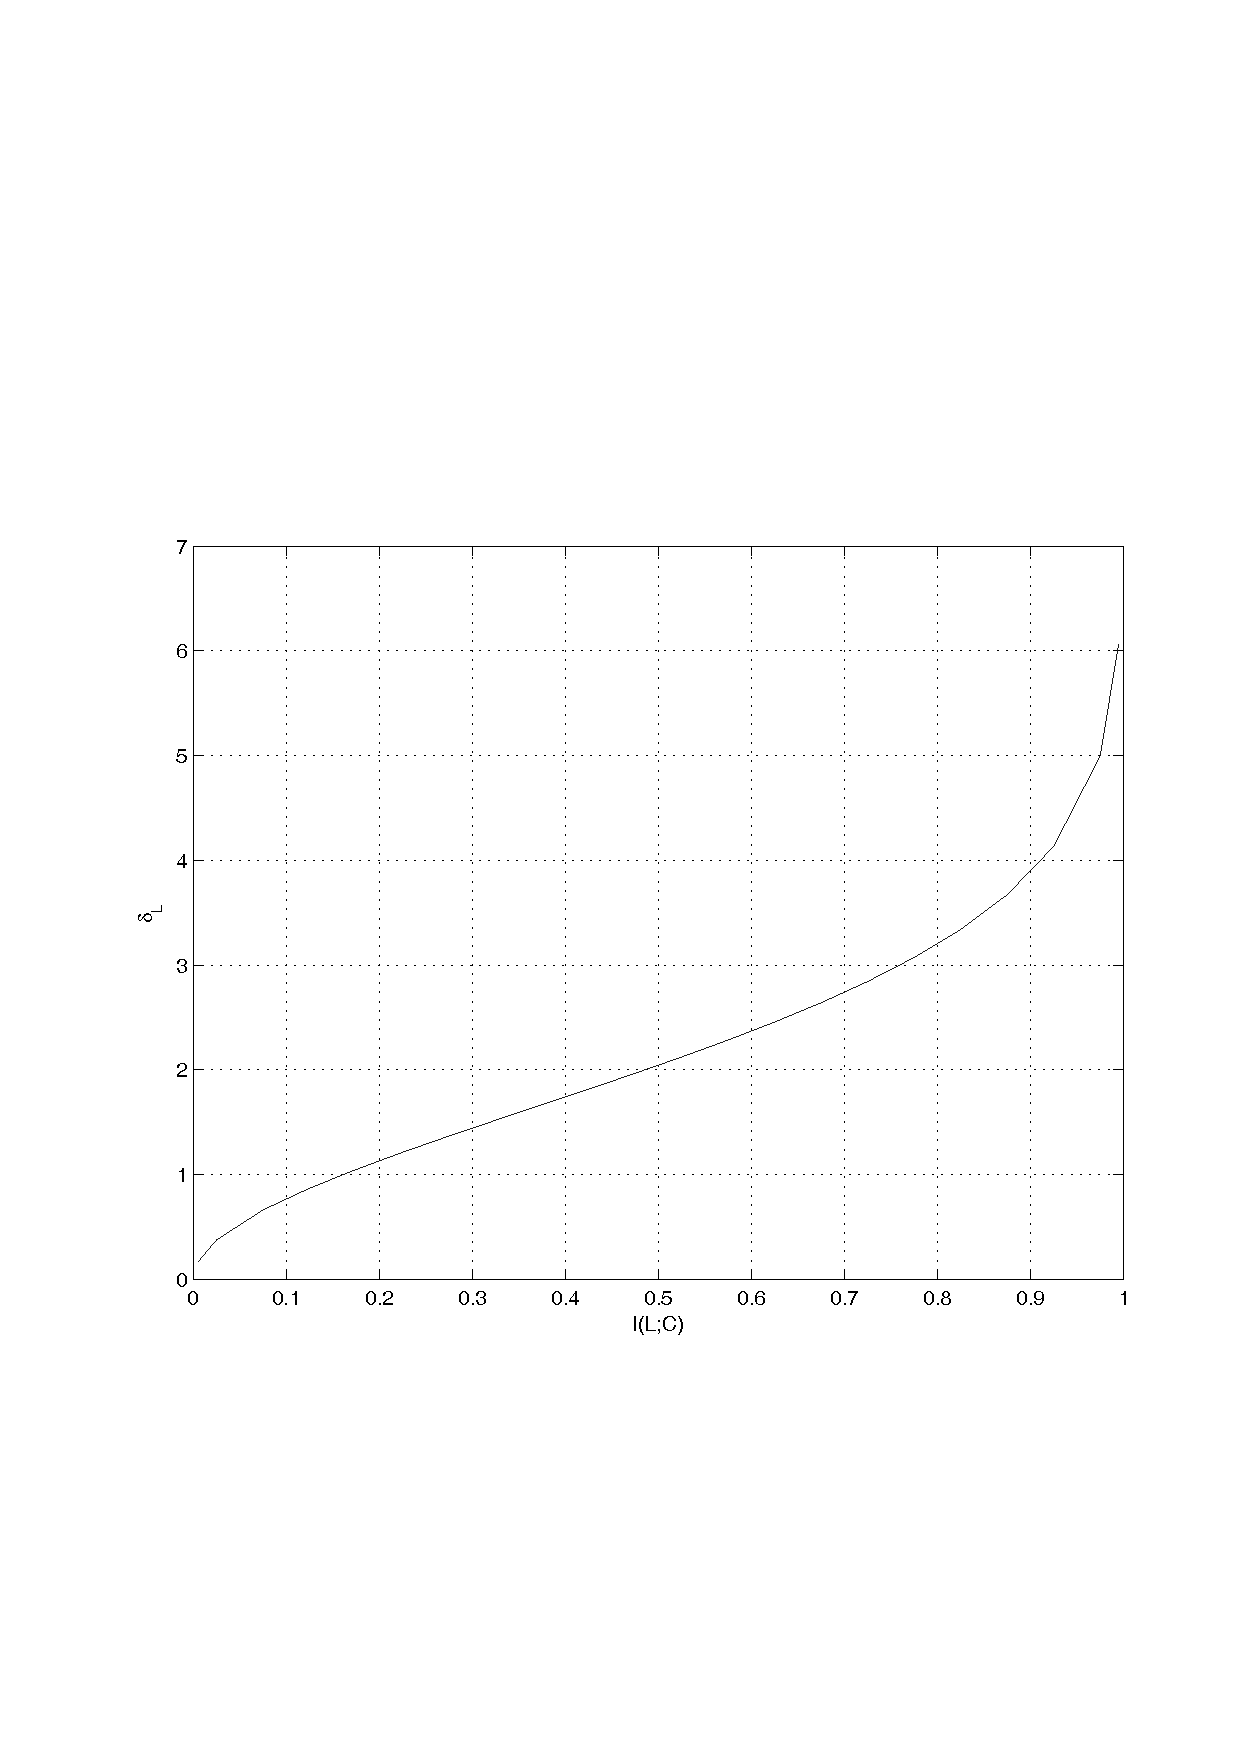
\includegraphics[width=0.8\textwidth]{images/relation.pdf}
  \end{center}
  \caption{互信息与$\sigma_L$的关系图}
  \label{fig:4.2}
\end{figure}
如图\ref{fig:4.2},当$\sigma_L=0$时,译码器反馈的软信息$L_e^D(c_{n,j})=0$,非常差,因为基本不提供任何的可靠性,而随着$\sigma_L$的增大,译码器反馈的软信息越来越可靠。

根据式(\ref{equ:3.7})-(\ref{equ:3.9}),利用译码器反馈的关于比特的$L_e^D(c_{n,j})$,可以得到每个符号的$y_{{n}'}$的均值$\bar{y_{{n}'}}$和方差$\upsilon_{y_{{n}'}}=\mathrm{E}(y_{{n}'}y_{{n}'}^*)$。利用统计量$\bar{y}_{{n}'}$和$\upsilon_{y_{{n}'}}$,发送符号$x_n$可以表示为:
\begin{eqnarray}
    x_n=\bar{x}_n+\chi_n
    \label{equ:4.3}
\end{eqnarray}
其中$\chi_n$为均值为零方差为$\mathrm{E}(\chi_n\chi_n^*)=\upsilon_n$的离散噪声。当传输的是数据符号时,可知,$\bar{x}=\bar{y}_{{n}'}$和$\upsilon_n=\upsilon_{y_{{n}'}}$。当传输的是训练序列的时候,$\bar{x}_n=t_n$和$\upsilon_n=0$。假设当$k\neq
n$的时候,$\mathrm{E}(\chi_n\chi_k^*)=0$(由于在turbo均衡中引入了交织器,因此上述假设是可以成立的),那么利用译码器反馈的软信息$L_e^D(c_{n,j})$得到的关于发送符号$x_n$协方差矩阵就是对角矩阵$\mathbf{V}_n=\mathrm{diag}[\upsilon_n,\cdots,\upsilon_{n-\mathrm{M}+1}]$。由式(\ref{equ:4.3})可知:
\begin{eqnarray}
    \mathrm{E}(\boldsymbol{\chi}_n\boldsymbol{\chi}_n^{\mathrm{H}})=\mathbf{V}_n
    \label{equ:4.4}
\end{eqnarray}
为了后文的仿真部分的比较,本章将考虑硬迭代信道估计算法。该算法利用通过硬判决符号$\tilde{x}_n$参与均衡器的迭代过程。

相较于文献\ncite{Brink2001,Nefedov2003,Otnes2004,Sandell1998,Qichenhao2011}中的信道估计算法,本文提出的软迭代信道估计算法不仅仅提供每个时刻的时变信道冲击响应的估计值$\hat{\mathbf{h}}_n$,而且还给出每个时候的相位估计值$\hat{\varphi}_n$。下面给出真实误差,软迭代误差以及硬迭代误差:
\begin{eqnarray}
    \begin{array}{l@{\;=\;}l}
        e_{m,n}&z_m-\hat{\mathbf{h}}_n^{\mathrm{T}}\mathbf{x}_me^{\imath\varphi_n}\\
        d_{m,n}&z_m-\hat{\mathbf{h}}_n^{\mathrm{T}}\bar{\mathbf{x}}_me^{\imath\hat{\varphi}_n}\\
        {d}'_{m,n}&z_m-\hat{\mathbf{h}}_n^{\mathrm{T}}\tilde{\mathbf{x}}_me^{\imath\tilde{\varphi}_n}\\
    \end{array}
    \label{equ:4.5}
\end{eqnarray}
其中$m$为误差信号所在时刻,$n$为估计的信道冲击响应所在时刻,$\mathbf{x}_n=[x_n,\cdots,x_{n-\mathrm{M}+1}]^{\mathrm{T}}$为期望发送符号序列,$\bar{\mathbf{x}}_n=[\bar{x}_n,\cdots,\bar{x}_{n-\mathrm{M}+1}]^{\mathrm{T}}$为软符号序列而$\tilde{\mathbf{x}}_n=[\tilde{x}_n,\cdots,\tilde{x}_{n-\mathrm{M}+1}]$为硬判决符号序列。下文中采用如下的简记方式$e_n=e_{n,n-1}\mbox{,}d_n=d_{n,n-1}\mbox{,}{d}'_n={d}'_{n,n-1}$。
%==========================================================================
\section{软迭代信道估计算法}
本文提出的软迭代信道估计算法包括两部分:软迭代横向滤波器系数估计算法和相位估计算法。由于采用此种幅度与相位分别估计的算法,因此各个部分可以针对水声信道的特点采用不同的算法。下面就对这两方面算法给出详细介绍。
%**************************************************************************
\subsection{软迭代横向滤波器系数估计算法}
%--------------------------------------------------------------------------
\subsubsection*{软迭代LMS横向滤波器系数估计算法}
最简单的信道估计算法为LMS,此时信道冲击响应估计值$\hat{\mathbf{h}}_n$按如下方式更新:
\begin{eqnarray}
    \hat{\mathbf{h}}_n=\hat{\mathbf{h}}_{n-1}+\beta e_n\mathbf{x}_n^*
    \label{equ:4.6}
\end{eqnarray}
其中参数$\beta$为步长因子,它的大小决定了算法的收敛速度和稳定性。一般来说,$\beta$越大收敛速度越快,但是稳定性越差,反之亦然。因此,在实际应用LMS算法时,步长因子$\beta$的选择至关重要。

但是LMS有个致命的问题:收敛速度慢。为了解决这个问题,有两种代替方案:1)最小二乘算法(RLS)算法。2)快速最优化算法(FOLMS)\citep{Geller1996}算法。FOLMS算法相比较与RLS算法由两个优点:(1)运算量小,与LMS算法的运算量基本一致。(2)稳定,RLS存在不稳定现象,影响系统的鲁棒性。基于以上分析,本文采用软迭代FOLMS信道估计算法。
%--------------------------------------------------------------------------
\subsubsection*{软迭代FOLMS横向滤波器系数估计算法(SIFOLMS)}
文献\ncite{Geller1996}给出了FOLMS信道均衡算法,本文在此基础上,将此算法应用到信道估计上并引入软迭代处理方式来提高算法的性能。

估计的接收信号为:
\begin{eqnarray}
    \bar{z}_n=\bar{\mathbf{x}}_n^{\mathrm{T}}\hat{\mathbf{h}}_{n-1}e^{\imath\hat{varphi}_{n-1}}
    \label{equ:4.7}
\end{eqnarray}
其中$\bar{\mathbf{x}}_n=[\bar{x}_k,\cdots,\bar{x}_{n-\mathrm{M}+1}]^{\mathrm{T}}$为利用式(\ref{equ:3.7})得到的软符号序列($n$时刻)。$\hat{\mathbf{h}}_{n-1}$为$n-1$时刻信道冲击响应的估计值(也即是横向滤波器系数估计值),$\hat{\varphi}_{n-1}$为信道的相位估计值。

均方误差定义如下:
\begin{eqnarray}
    J(\hat{\mathbf{h}},\hat{\varphi})=\mathrm{E}(|e_n|)^2
    \label{equ:4.8}
\end{eqnarray}
其中$e_n=z_n-\bar{z}_n$,$\bar{z}_n$为利用式(\ref{equ:4.7})得到的信道估计器输出,$z_n$为接收到的符号。

LMS算法中一般采用最陡下降法来减少计算量,而FOLMS本质上是基于LMS算法,因此,也可以利用最陡下降法。$J$针对于$\hat{\mathbf{h}}$的梯度为:
\begin{eqnarray}
    \nabla_{\hat{\mathbf{h}}}|e_n|^2=-2\bar{\mathbf{x}}_n^*e^{-\imath\hat{\varphi}}e_n
    \label{equ:4.9}
\end{eqnarray}
因此$\hat{\mathbf{h}}_n$的更新方程为:
\begin{eqnarray}
    \hat{\mathbf{h}}_n=\bar{\mathbf{h}}_{n-1}+\mu\bar{\mathbf{x}}_n^*e^{-\imath\hat{\varphi}_{n-1}}e_n
    \label{equ:4.10}
\end{eqnarray}
其中$e_n=z_n-\bar{\mathbf{x}}_n^{\mathrm{T}}\hat{\mathbf{h}}_{n-1}e^{\imath\hat{\varphi}_{n-1}}$。

在信道未知的情况下,合理的步长因子$\mu$的选取非常困难,为了减少算法对于步长因子选择的依赖性,采用步长因子自适应调整方案。

稳态均方误差$J$依赖于步长因子$\mu$,因此可以改写为:
\begin{eqnarray}
    J(\mu)=\lim_{n\rightarrow\infty}\mathrm{E}(|z_n-\bar{\mathbf{x}}_n^{\mathrm{T}}\hat{\mathbf{h}}_{n-1}e^{\imath\hat{\varphi}_{n-1}}|^2)
    \label{equ:4.11}
\end{eqnarray}

现在的目标是在式(\ref{equ:4.10})的约束条件下,通过调整$\mu$来最小化式(\ref{equ:4.10})。将式(\ref{equ:4.10})和(\ref{equ:4.11})联合,可以改写均方误差$J$如下:
\begin{eqnarray}
    J(\bar{\mathbf{x}}_n,z_n,\hat{\mathbf{h}}_{n-1},\hat{\varphi}_{n-1},\mu)=|z_k-\bar{\mathbf{x}}_n\hat{\mathbf{h}}_{n-1}e^{\imath\hat{\varphi}_{n-1}}|^2
    \label{equ:4.12}
\end{eqnarray}
并令:
\begin{eqnarray}
    \mathbf{G}_n=\frac{\partial\hat{\mathbf{h}}_n}{\partial\mu}
    \label{equ:4.13}
\end{eqnarray}
根据最陡下降法可以得出步长因子$\mu$的更新方程:
\begin{eqnarray}
    \begin{array}{l@{\;=\;}l}
    \mu_n&\mu_{n-1}-\beta\frac{\partial J}{\partial\mu}\\
    &\mu_{n-1}-\beta\mathrm{Re}(\bar{\mathbf{x}}_n^{\mathrm{H}}\exp(\imath\hat{\varphi}_{n-1})\mathbf{G}_{n-1}e_n)
    \end{array}
    \label{equ:4.14}
\end{eqnarray}
引入关于步长因子$\mu(\mu_{\max},\mu_{\min})$的最大值和最小值这一约束条件之后,步长因子$\mu$的更新方程如下:
\begin{eqnarray}
    \mu_n=[\mu_{n-1}-\beta\mathrm{Re}(\bar{\mathbf{x}}_n^{\mathrm{H}}\mathbf{G}_{n-1}e^{\imath\hat{\varphi}_{n-1}}e_n)]_{\mu_{\min}}^{\mu_{\max}}
    \label{equ:4.15}
\end{eqnarray}
其中,$\beta$为$\mu$的步长因子且
\begin{eqnarray}
    \mathbf{G}_n=(\mathbf{I}-\mu_n\bar{\mathbf{x}}_n^*\bar{\mathbf{x}}_n^{\mathrm{T}})\mathbf{G}_{n-1}+\bar{\mathbf{x}}_{n}^*e_n
    \label{equ:4.16}
\end{eqnarray}

文献\ncite{Geller1996}指出,步长因子$\beta$可以选择的范围非常大且性能基本没有损失。在实际应用中,为了系统的稳定性,$\mu_n$一般限定在其最大值和最小值之间。式(\ref{equ:4.7}),式(\ref{equ:4.10}),式(\ref{equ:4.15})以及式(\ref{equ:4.16})构成软迭代横向滤波器抽头系数估计算法。
%**************************************************************************
\subsection{相位估计算法}
针对水声信道多普勒效应严重的现象,采用单独的相位估计算法,目前实际应用与水声系统中的估计算法常用的为二阶锁相环相位估计算法。下面就对这这种算法进行介绍。
%--------------------------------------------------------------------------
\subsubsection*{二阶锁相环相位估计算法(PLLPC)}
文献\ncite{Stojanovic1994}给出二阶锁相环在水声通信系统的鉴相器方程以及相位更新方程:
\begin{eqnarray}
    \begin{array}{l@{\;=\;}l}
    \Psi_n=\mathrm{Im}(\bar{z}_nz_n^*)\\
    \hat{\varphi}_{n+1}=\hat{\varphi}_n+K_1\Psi_n+K_2\sum\limits_{i=0}^n\Psi_i
    \end{array}
    \label{equ:4.21}
\end{eqnarray}
其中$\bar{z}_n=\bar{\mathbf{x}}_n^{\mathrm{T}}\hat{\mathbf{h}}_{n-1}e^{\imath\hat{\varphi}_{n-1}}$,$K_1$和$K_2$为二阶锁相环的两个参数。$K_1=2\xi w_c\mbox{,}K_2=w_c^2$,$\xi$为环路阻尼系数,$\xi>1$比$\xi<1$的系统更稳定,但是对输入变化的响应更迟缓,为了平衡稳定性和响应速度,二阶锁相环通常取$\xi\approx
1/\sqrt{2}$。而$w_c$为归一化自然角频率,例如$w_c=0.001$,则:$K_1=1.4\times
10^{-3}\mbox{,}K_2=1\times 10^{-6}$。

表\ref{tab:4.1}是SIFLOMS-PLLPC算法的总结。
\begin{table}[hbt]
  \centering
  \caption{软迭代信道估计算法总结}
  \label{tab:4.1}
  \begin{threeparttable}
  \begin{tabular}{c}
    \hline
    SIFOLMS-PLLPC\\
    \hline
    $
    \begin{array}{l@{\;=\;}l}
        \bar{z}_n&\bar{\mathbf{x}}_n^{\mathrm{T}}\hat{\mathbf{h}}_{n-1}e^{\imath\hat{\varphi}_{n-1}}\\
        e_n&z_n-\bar{z}_n\\
        \hat{\varphi}&\hat{\varphi}_{n-1}+K_1\Psi_{n-1}+K_2\sum\limits_{i=0}^{n-1}\Psi_i\\
        \Psi_n&\mathrm{Im}(\bar{z}_nz_n^*)\\
        \hat{\mathbf{h}}_n&\hat{\mathbf{h}}_{n-1}+\mu_{n-1}\bar{\mathbf{x}}_{n}^*e^{-\imath\hat{\varphi}_{n-1}}\\
        \mu_n&[\mu_{n-1}-\beta\mathrm{Re}(\bar{\mathbf{x}}_n^{\mathrm{H}}\mathbf{G}_{n-1}e^{\imath\hat{\varphi}_{n-1}}e_n)]_{\mu_{\min}}^{\mu_{\max}}\\
        \mathbf{G}_n&(\mathbf{I}-\mu_n\bar{\mathbf{x}}_n^*\bar{\mathbf{x}}_n^{\mathrm{T}})\mathbf{G}_{n-1}+\bar{\mathbf{x}}_n^*e^{-\imath\hat{\varphi}_n}e_n\\
    \end{array}
    $\\
    \hline
  \end{tabular}
\end{threeparttable}
\end{table}

从表\ref{tab:4.1}中可以看出,FOLMS算法和二阶锁相环算法均没有增加信道估计的运算复杂度,因此复杂度与LMS算法基本一致。
%**************************************************************************
\subsection{方差估计}
在第三章中为了推导已知信道条件下的SISO均衡算法,采用的信道模型是:
\begin{eqnarray}
    z_n=\mathbf{h}_n^{\mathrm{T}}\mathbf{x}_n+\omega_n
    \label{equ:4.22}
\end{eqnarray}
其中$\omega_n$是均值为零方差为$\sigma_{\omega,n}^2$\footnote{方差是时变的,且在求解SISO均衡器系数时要求知道该值}的复高斯变量。当信道为时变未知的时候,式(\ref{equ:4.22})将会被下式所替代:
\begin{eqnarray}
    z_n=\hat{\mathbf{h}}_{n-1}^{\mathrm{T}}\mathbf{x}_n+e_n
    \label{equ:4.23}
\end{eqnarray}
从上式可以发现,信道冲击响应$\mathbf{h}_n$被估计的信道冲击响应值$\hat{\mathbf{h}}_{n-1}$所替代,而噪声信道$\omega_n$被误差信号$e_n$所替代,当然噪声的方差$\sigma_{\omega,n}$也相应的被$e_n$的方差$\sigma_{e,n}$所替代。但问题的关键在于方差$\sigma_{e,n}$是未知的,因此需要对该方差进行估计:
\begin{eqnarray}
    \hat{\sigma}_{e,n}^2\approx\sigma_{e,n}^2=\mathrm{E}(e_ne_n^*)
    \label{equ:4.24}
\end{eqnarray}
如果发送符号$x_n$都是已知的,那么此时就可以很容易的得到方差$\hat{\sigma}_{e,n}^2$,但是在软迭代信道估计算法中,已知的只有关于发送符号的先验均值$\bar{x_n}$和方差$\upsilon_n$,因此信道模型可以改写如下:
\begin{eqnarray}
    z_n=\hat{\mathbf{h}}_{n-1}^{\mathrm{T}}\bar{\mathbf{x}}_n+d_n
    \label{equ:4.25}
\end{eqnarray}
此时,可以利用误差信号$d_n$来估计$\sigma_{e,n}^2$。

目前,对于如何从误差信号$d_n$来估计方差并没有一种很好的方法,文献\ncite{Otnes2004}给出一种递归求解方式,本文与其算法不同之处在于需要加入估计的相位值。
\begin{itemize}
    \item \heiti 初始化:\begin{eqnarray}
            \hat{\sigma}_{e,0}^2=\hat{\sigma}_{\mathrm{init}}^2
            \label{equ:4.26}
        \end{eqnarray}
    \item 在训练符号($\mathbf{V}_n=\mathbf{0}_{\mathrm{M}}$)时:
        \begin{eqnarray}
            \begin{array}{l@{\;=\;}l}
                \hat{\sigma}_{e,n}^2&\mu_{n}
                d_nd_n^*+(1-\mu_{n})\hat{\sigma}_{e,n-1}^2\\
                \hat{\sigma}_{\mathrm{low}}^2&\hat{\sigma}_{e,n}^2
            \end{array}
            \label{equ:4.27}
        \end{eqnarray}
    \item 在数据符号($\mathbf{V}_n\neq
        \mathbf{0}_{\mathrm{M}}$)时:
        \begin{eqnarray}
            \begin{array}{l@{\;=\;}l}
                \hat{\sigma}_{\mathrm{new}}^2&\mu_{n}(d_nd_n^*-\hat{\mathbf{h}}^{\mathrm{T}}_{n-1}\exp{\imath\hat{\psi}_{n-1}}\mathbf{V}_n\hat{\mathbf{h}}_{n-1}^*\exp{-\imath\hat{\psi}_{n-1}})+(1-\mu_{n})\hat{\sigma}_{e,n-1}^2\\
                \hat{\sigma}_{e,n}^2&\max(\hat{\sigma}_{\mathrm{new}}^2,\hat{\sigma}_{\mathrm{low}}^2)
            \end{array}
            \label{equ:4.28}
        \end{eqnarray}
\end{itemize}
其中,$\mathbf{V}_n$为数据符号的协方差矩阵。
%**************************************************************************
\section{仿真分析}
本文软迭代信道估计算法的仿真信道基于时变横向滤波和相位旋转信道模型。时变横向滤波的阶数为5,各抽头系数为独立的高斯随机过程,每阶系数采用白噪声作为激励的一阶自回归模型产生。生成公式为:
\begin{eqnarray}
    \mathbf{h}_n=(\rho\mathbf{h}_{n-1}+\sqrt{1-\rho^2}[q_{n,0},\cdots,q_{n,4}]^{\mathrm{T}})
    \label{equ:4.29}
\end{eqnarray}
其中,$\rho=\sqrt{0.999}$为衰落因子。$q_{n,i}$是均值为零方差为$1/5$的高斯随机变量,因此可以保证信道冲击响应的平均能量为一。信道冲击响应初始化为$\mathbf{h}_{0}=[1,1,\cdots,1]/\sqrt{5}$。对于相位旋转部分,通过对以往海试数据处理分析可知,由于船体随着波浪作类似简谐运动,因此相位也呈现出类似的变化规律:
\begin{eqnarray}
    \varphi=\frac{2\pi A}{\lambda}\sin(\frac{2\pi t}{T})
    \label{equ:4.30}
\end{eqnarray}
其中,$A$为船体运动的最大振幅,$\lambda$为波长,$T$为周期。对于7000m载人潜水器的通信系统以及20110730002719海试数据的海况来说,$A=5m$,$\lambda=c/f_c=1500/10000=0.15m$,其中,$c$为声速,$f_c$为载波频率,$T=10s$。海试数据在进入均衡器之前通常需要对其进行线性多普勒补偿,图\ref{fig:4.3}为经过线性多普勒补偿之后残留的相位变化曲线。本文选取变化幅度最大的一个相位变化曲线作为本文信道相位仿真模型,并建模成正弦函数来简化仿真。
\begin{figure}[htb]
  \begin{center}
    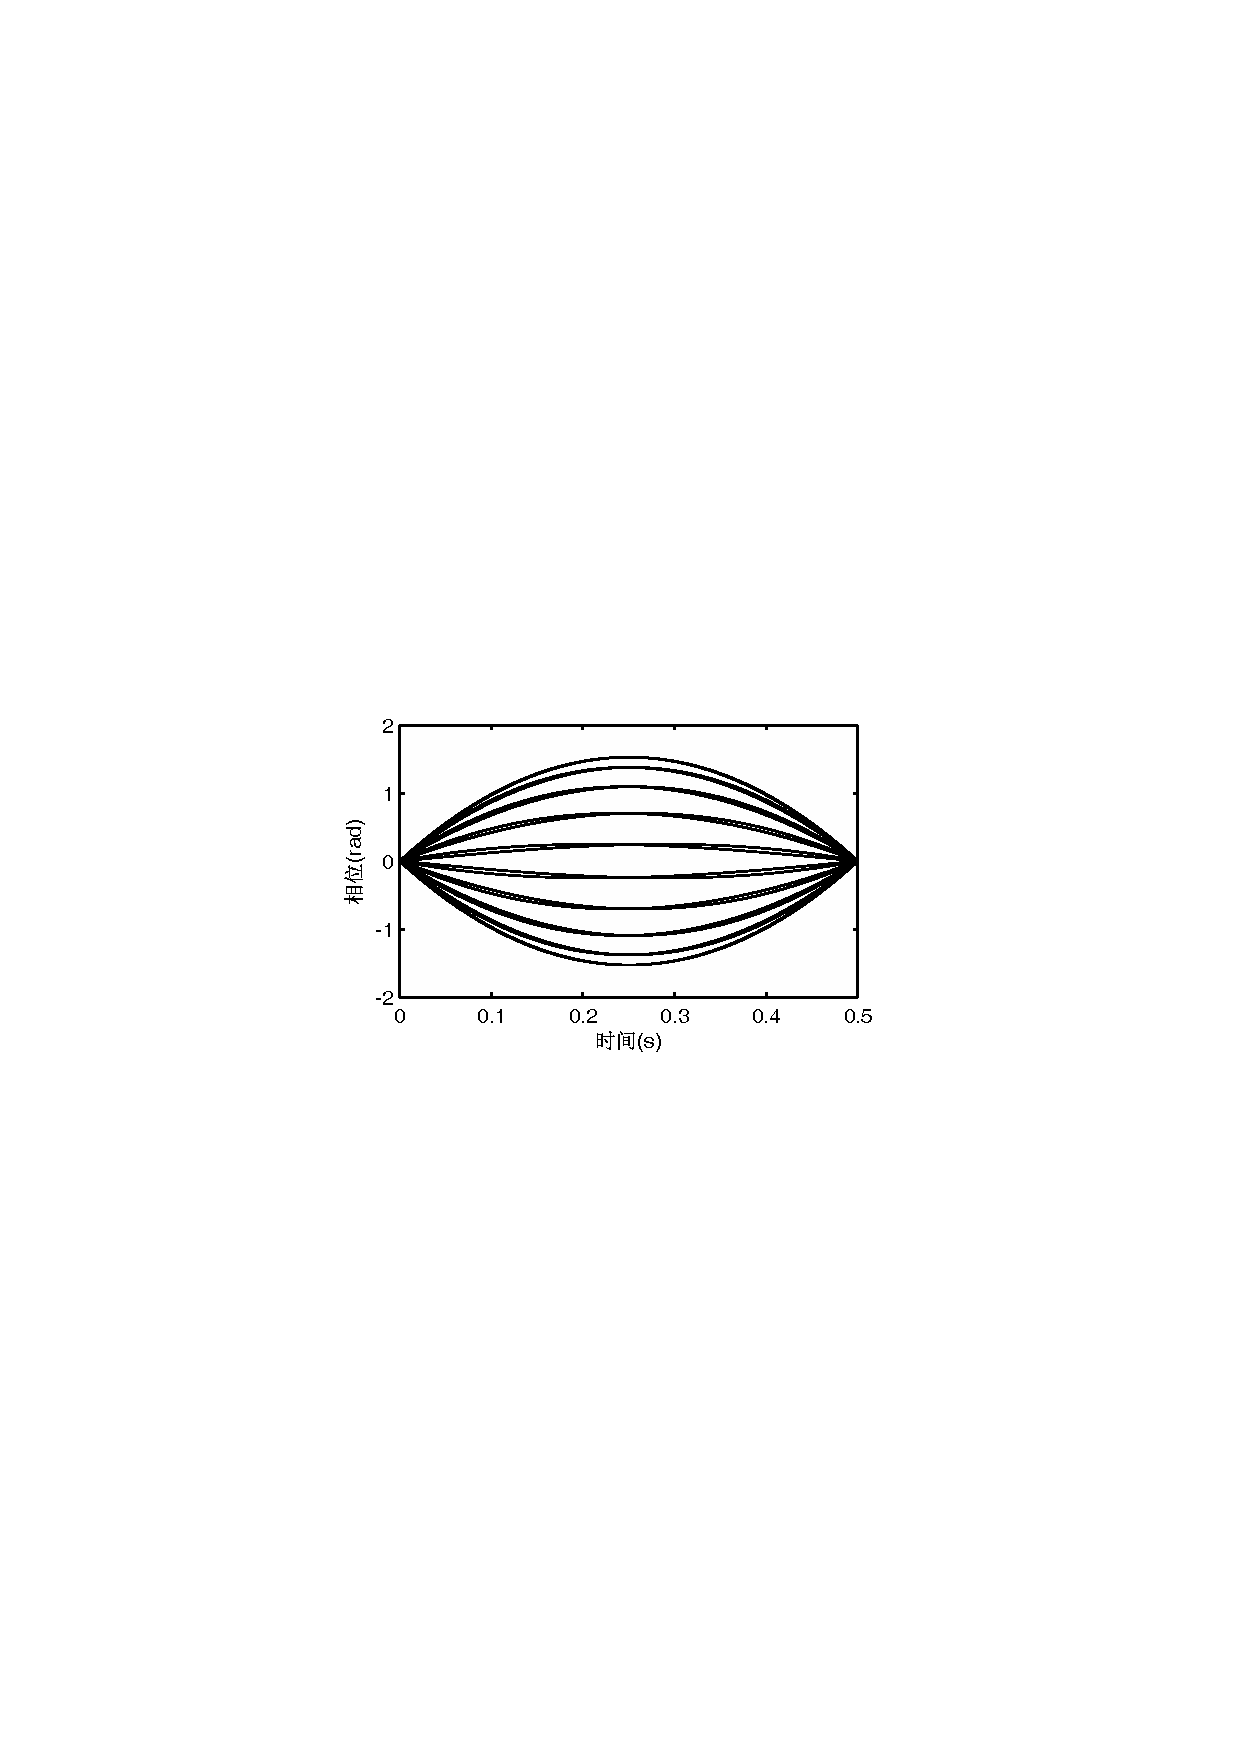
\includegraphics[width=0.9\textwidth]{images/phase_diff.pdf}
  \end{center}
  \caption{线性多普勒补偿后相位变化曲线}
  \label{fig:4.3}
\end{figure}

仿真参数设置如下:训练符号序列$\mathbf{t}_n$和通过$(23,35)$Turbo码生成的数据符号序列一起构成发送符号序列$\mathbf{x}_n$。一帧数据包含长度为$200$个符号的初始化训练序列,以及$9$个长度为$150$的数据符号和长度为$50$的内插训练符号。每一个传输符号$x_n$的能量$E_s$都被归一化。每一个信道估计算法都产生长度为$M={M}'+2=7$的时变信道冲击响应的估计值$\hat{\mathbf{h}}_n$(因为在信道估计的时候并不知道信道冲击响应${M}'$的确切值),方差的估计值$\hat{\sigma}_e^2$以及相位的估计值$\hat{\varphi}_n$。本文的仿真在信噪比为$E_b/N_0=10\mathrm{dB}$的条件下,执行$1000$帧。
\subsection{软硬迭代信道估计算法的比较}
传统信道估计算法引入迭代并将译码器判决的符号作为信道估计的期望符号,从而形成硬迭代信道估计算法。为了对比软迭代与硬迭代信道估计算法的性能,图\ref{fig:4.4}给出了在$\sigma_L=1$时硬迭代信道估计算法与软迭代信道估计算法的比较结果,下面从两个方面对图\ref{fig:4.4}所示的仿真结果加以分析。

\begin{figure}
    \centering
    \subfigure[硬迭代信道估计算法]{
    \centering\label{fig:4.4.a}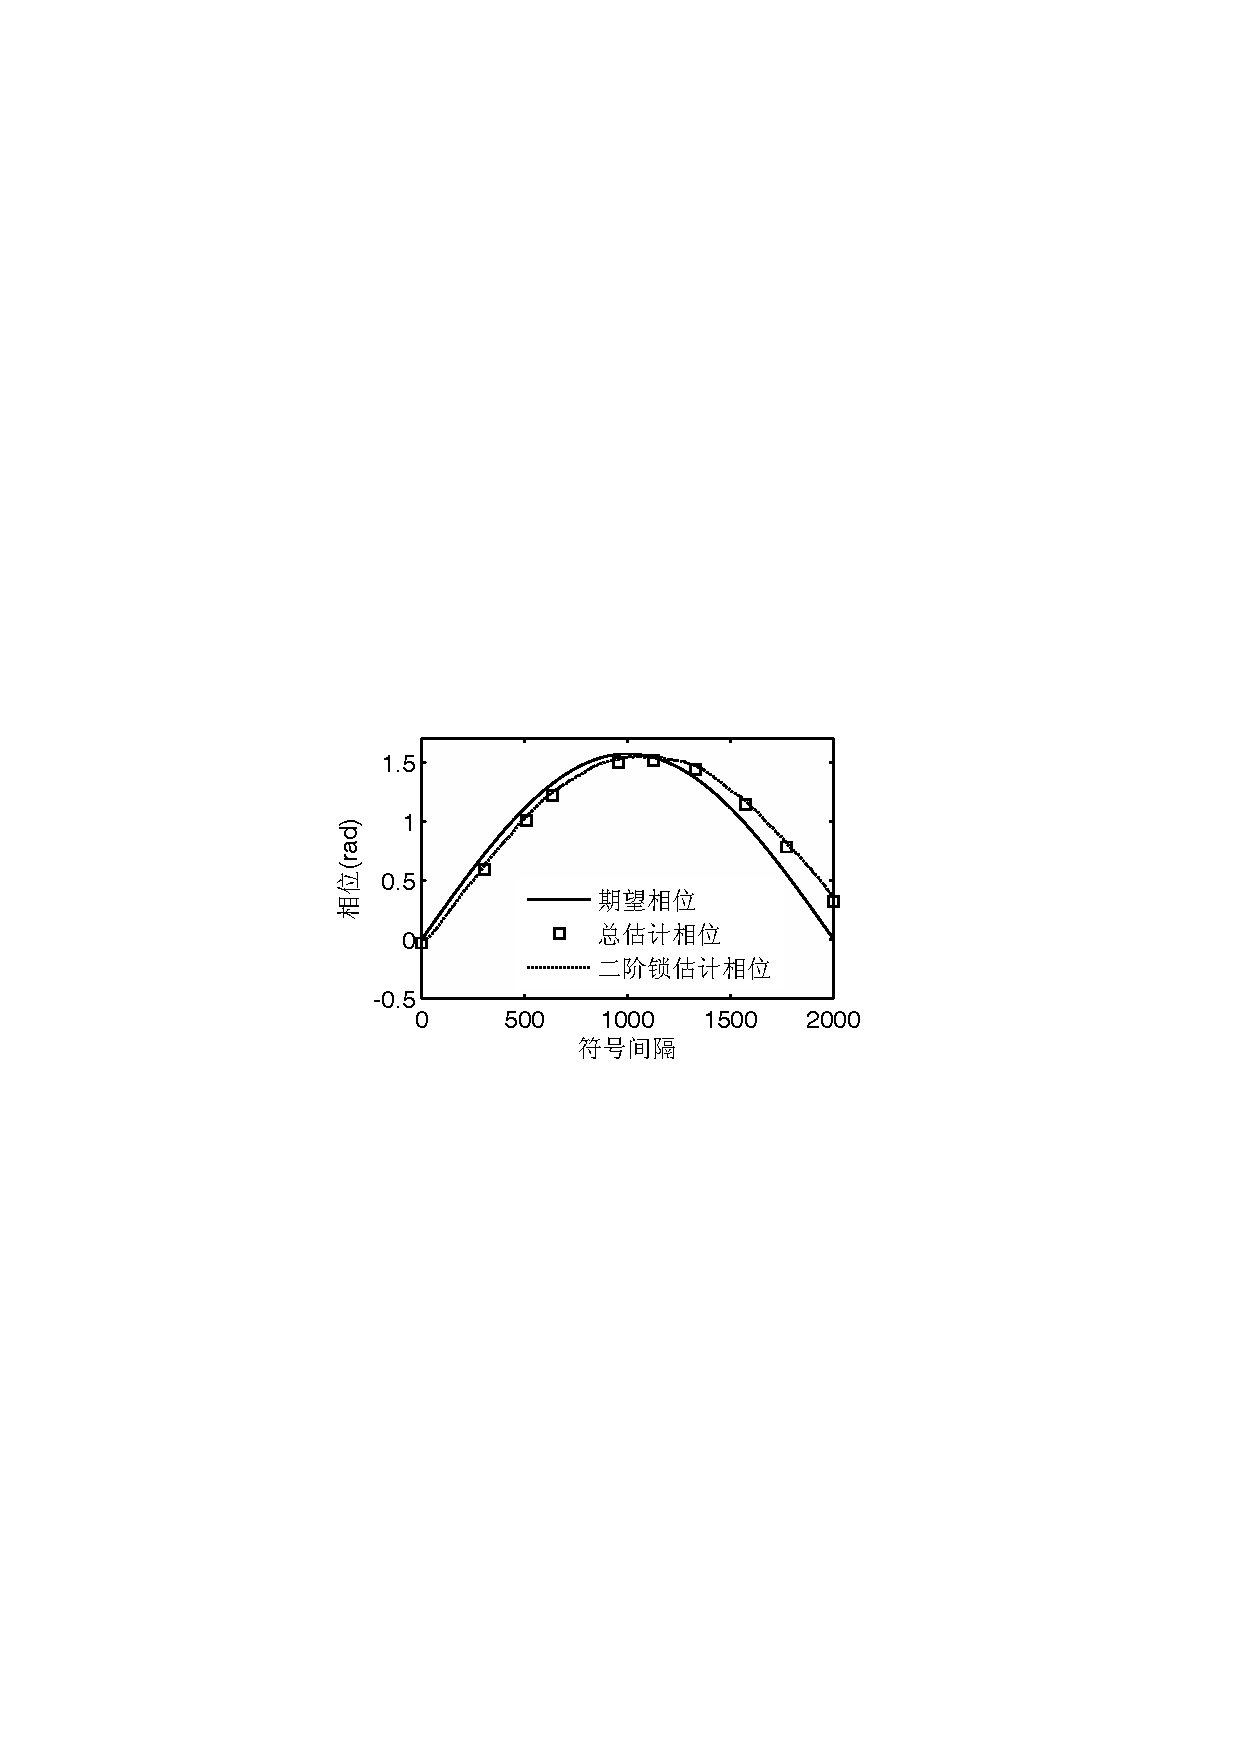
\includegraphics[width=0.45\textwidth]{images/hard_soft_1_a.pdf}
}
    \subfigure[软迭代信道估计算法]{
    \label{fig:4.4.b}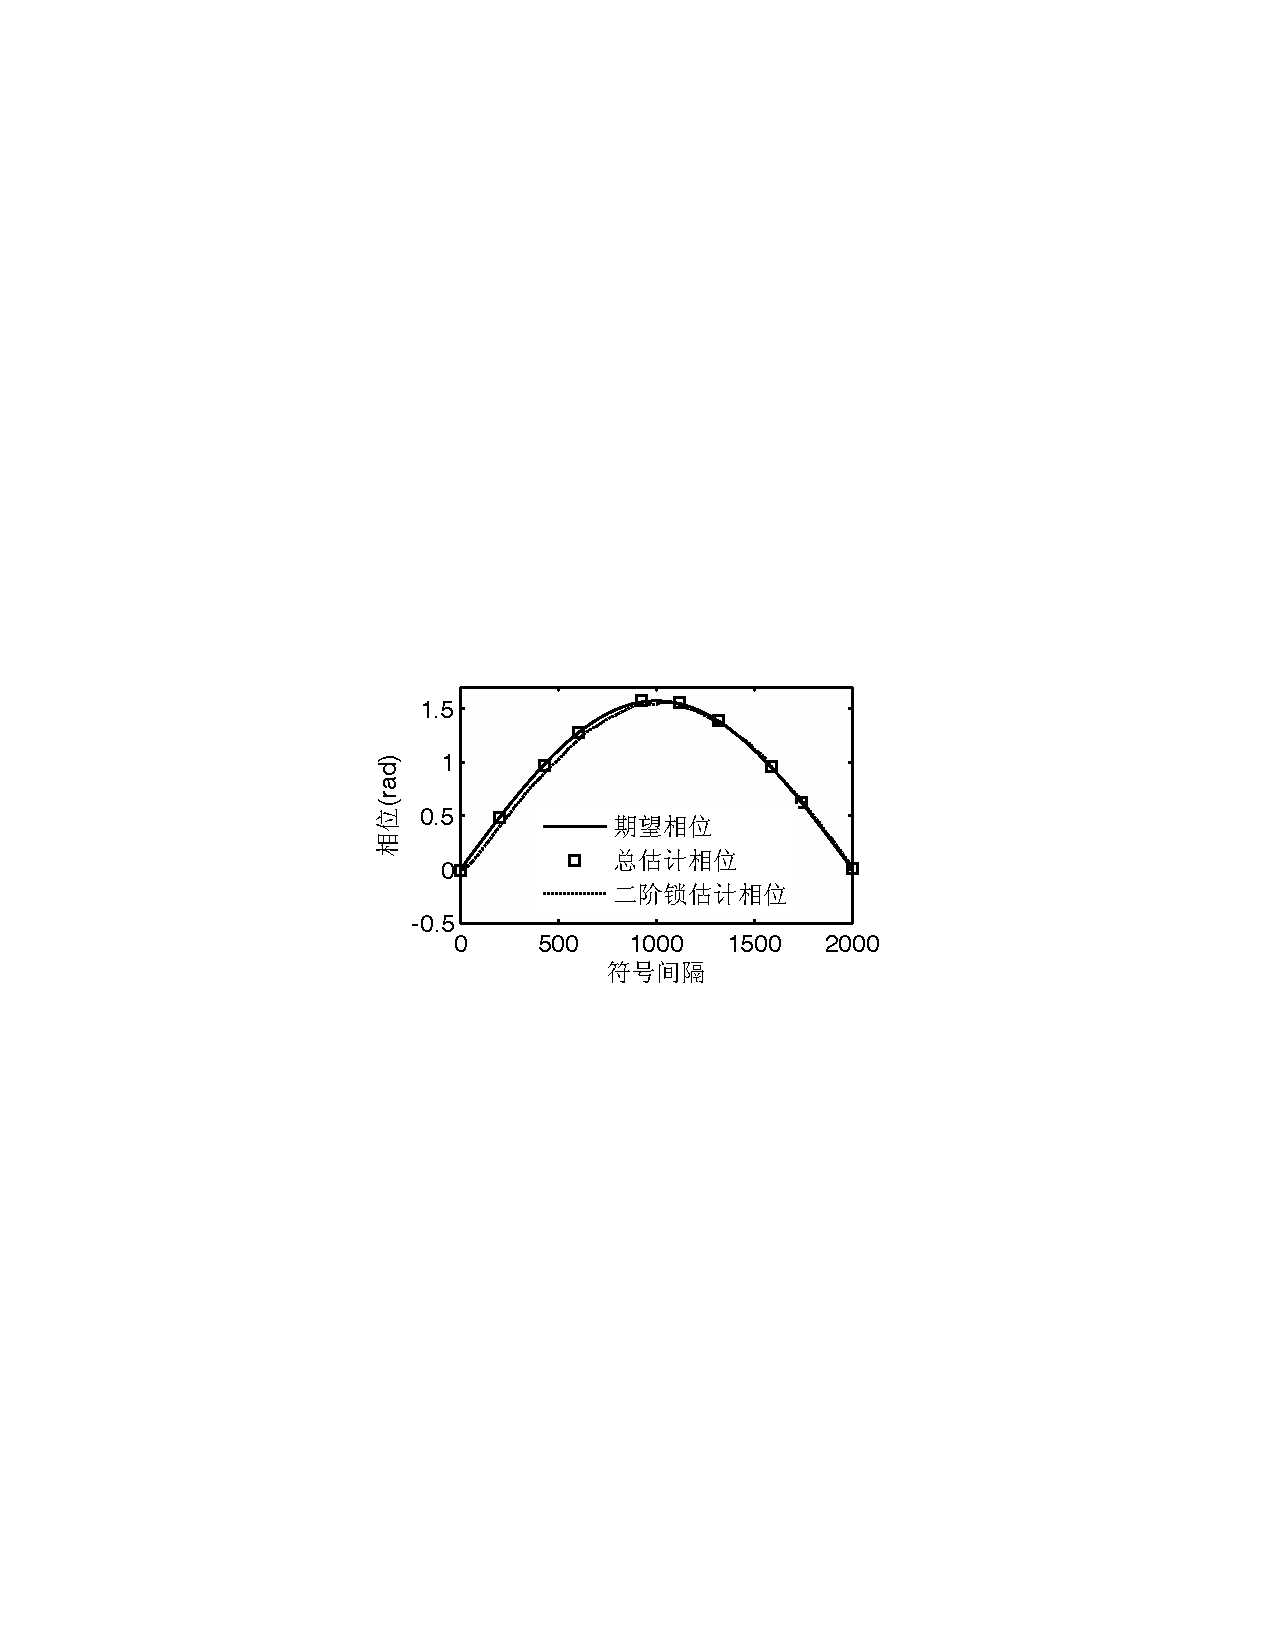
\includegraphics[width=0.45\textwidth]{images/hard_soft_1_b.pdf}
}\\
    \subfigure[信道方差估计]{
    \label{fig:4.4.c}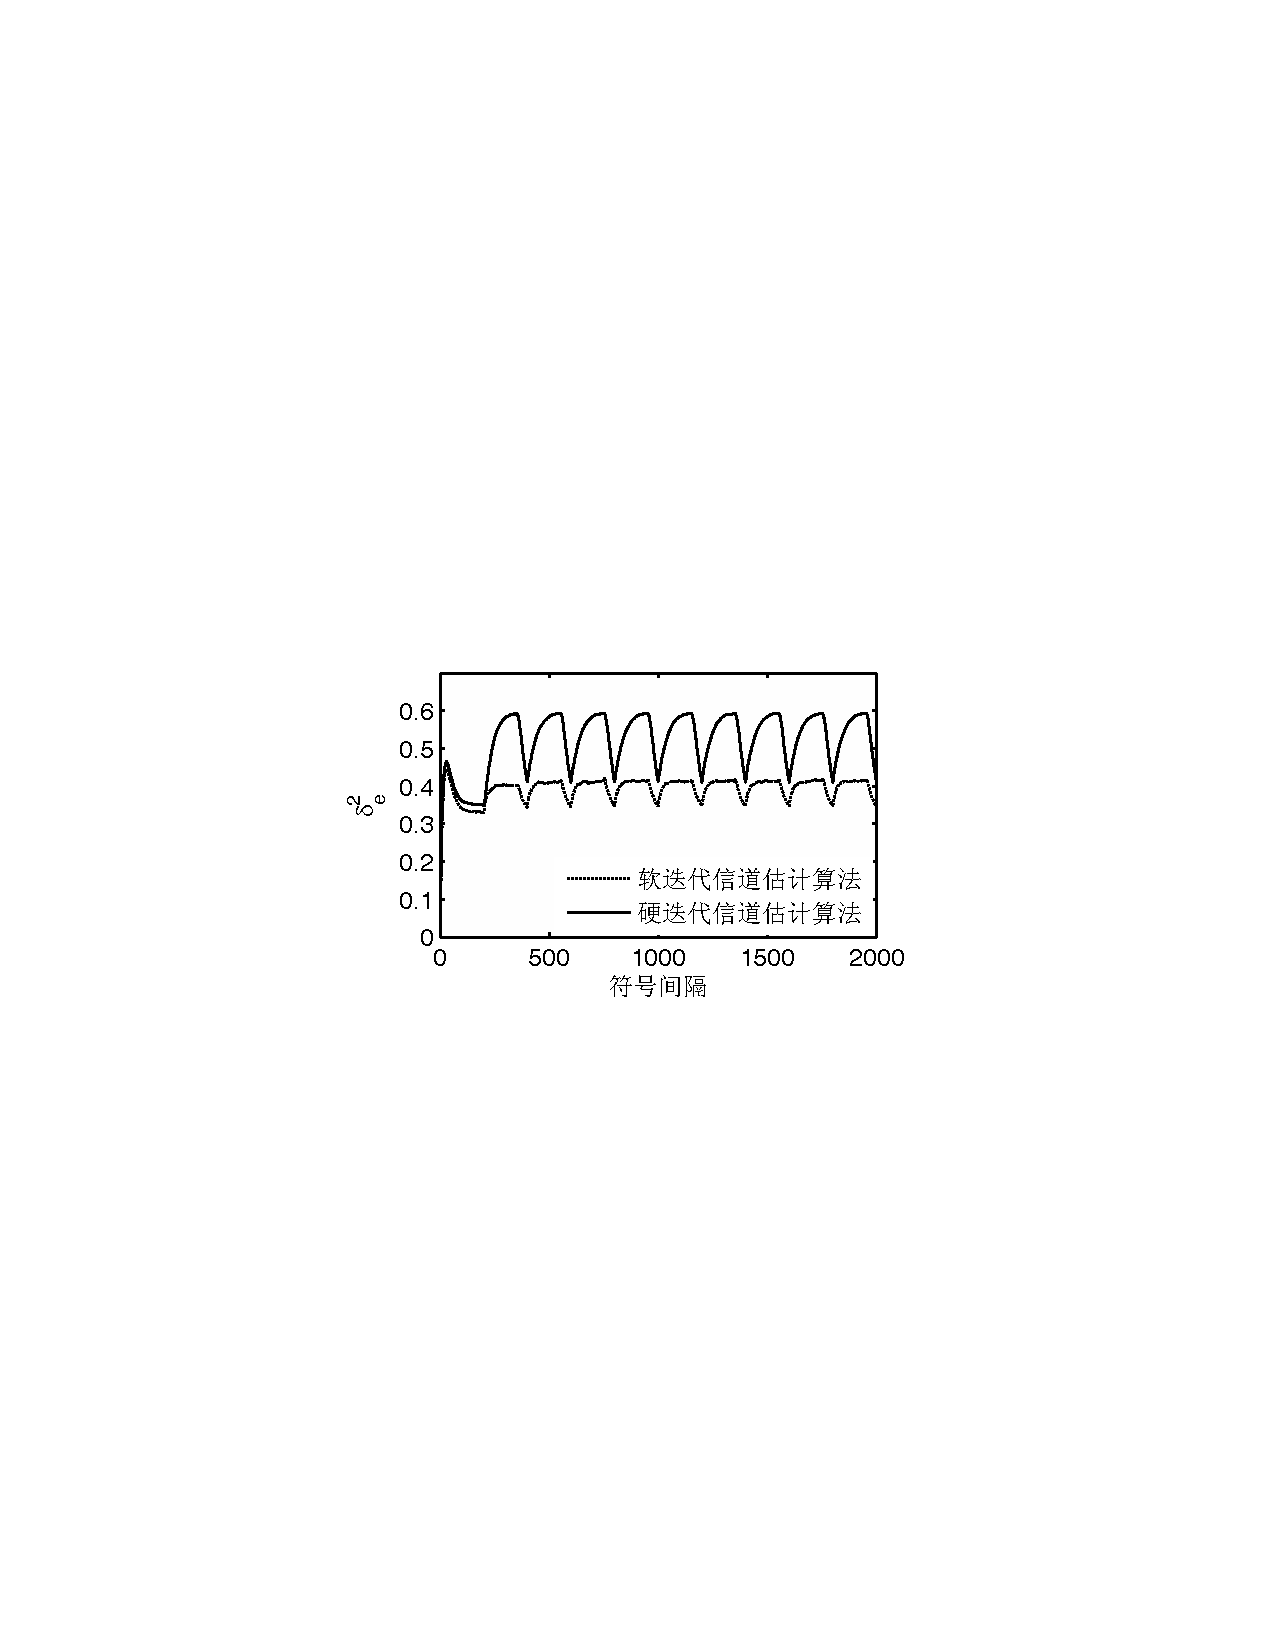
\includegraphics[width=0.5\textwidth]{images/hard_soft_1_c.pdf}
}%
    \caption{$\sigma_L=1$时硬迭代与软迭代信道估计算法比较}
    \label{fig:4.4}
\end{figure}
在相位估计方面,不论是单独的二阶锁相环的相位估计值还是总的相位估计值(二阶锁相环相位估计值+横向滤波器抽头系数中的相位值),软迭代信道估计算法都优于同等条件下的硬迭代信道估计算法。在信道方差$\sigma_e^2$估计方面,不论是软迭代信道估计算法还是硬迭代信道估计算法,当使用训练序列进行信道与相位估计时,$\sigma_e^2$值随着训练序列长度的增加而下降,而当使用数据符号时,$\sigma_e^2$随之增大。但是通过对整帧数据的观察可知,除去初始化训练序列外,在数据符号序列时,软迭代信道估计算法的方差$\sigma_e^2$要明显小于硬迭代信道估计算法的方差估计值。

\begin{figure}
    \centering
    \subfigure[硬迭代信道估计算法]{
    \centering\label{fig:4.5.a}\includegraphics[width=0.45\textwidth]{images/hard_soft_3_a.pdf}
}
    \subfigure[软迭代信道估计算法]{
    \label{fig:4.5.b}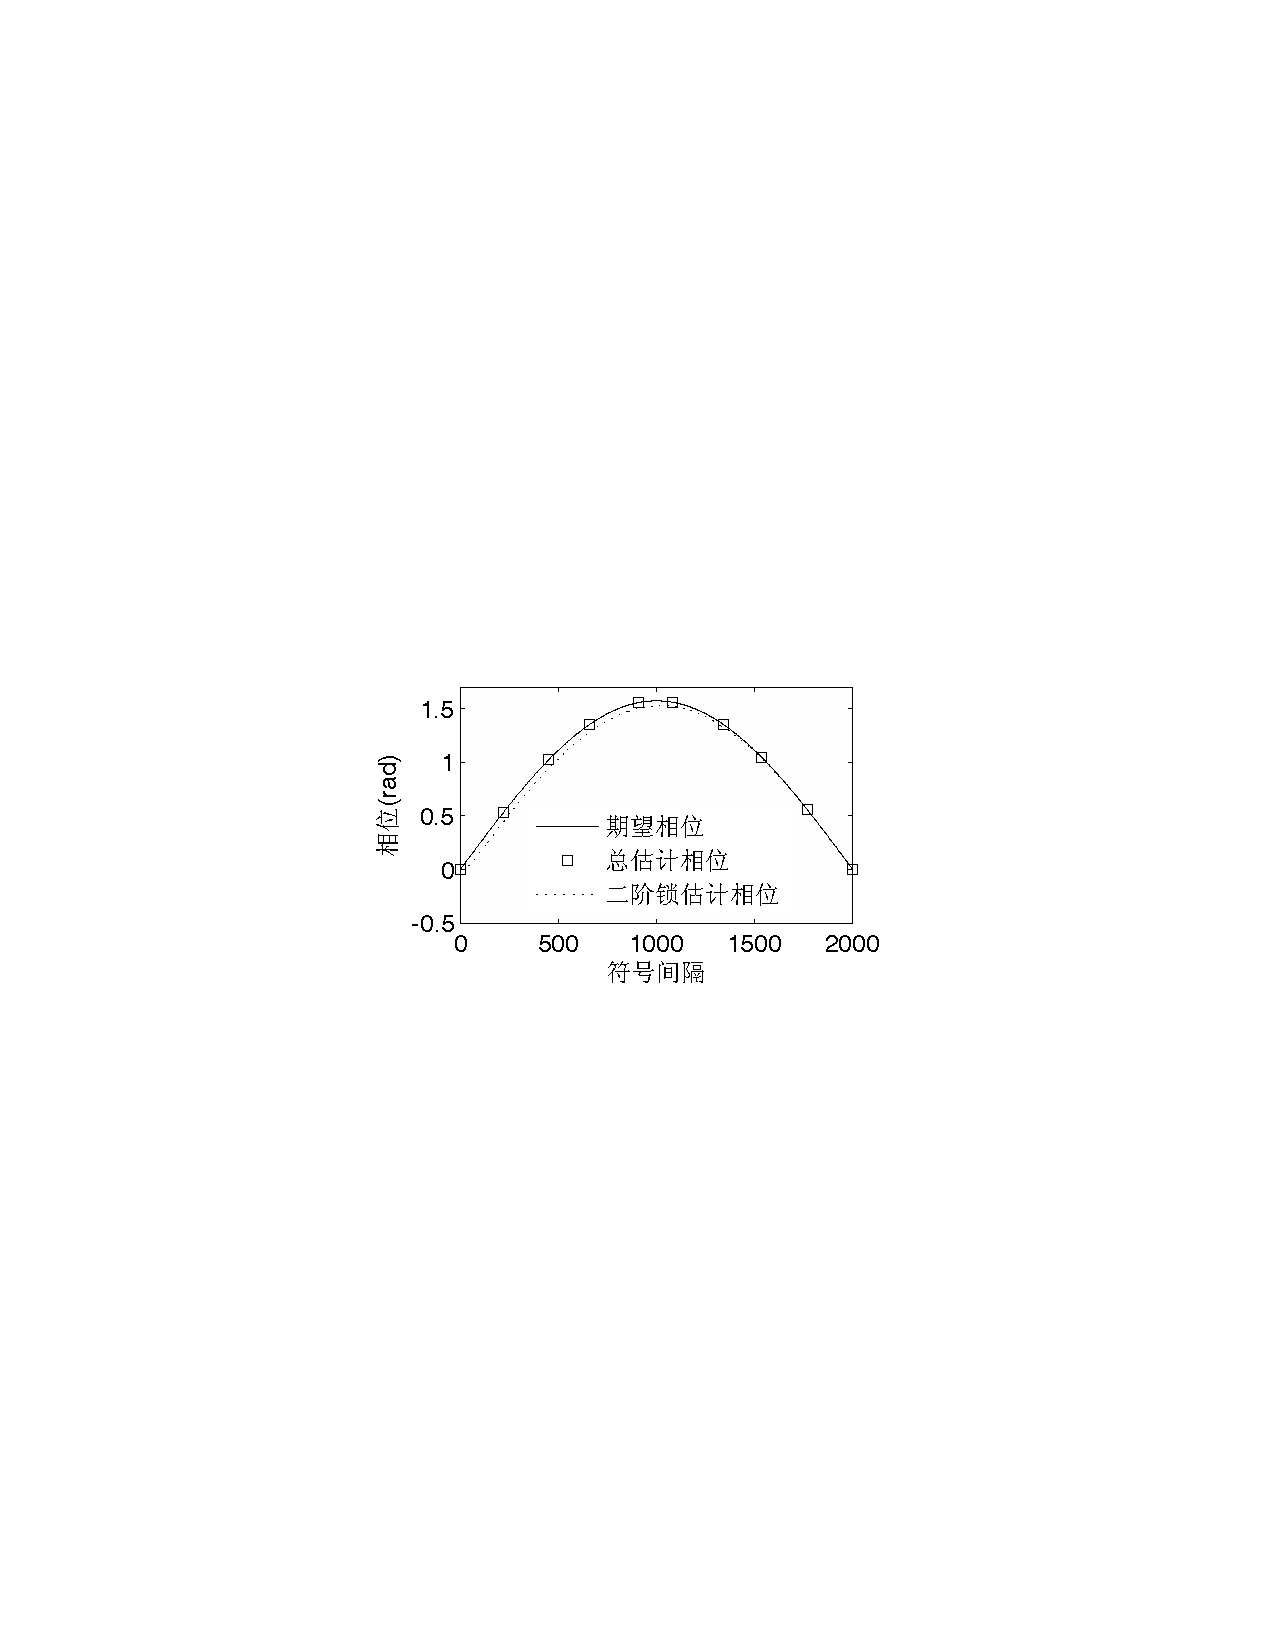
\includegraphics[width=0.45\textwidth]{images/hard_soft_3_b.pdf}
}\\
    \subfigure[信道方差估计]{
    \label{fig:4.5.c}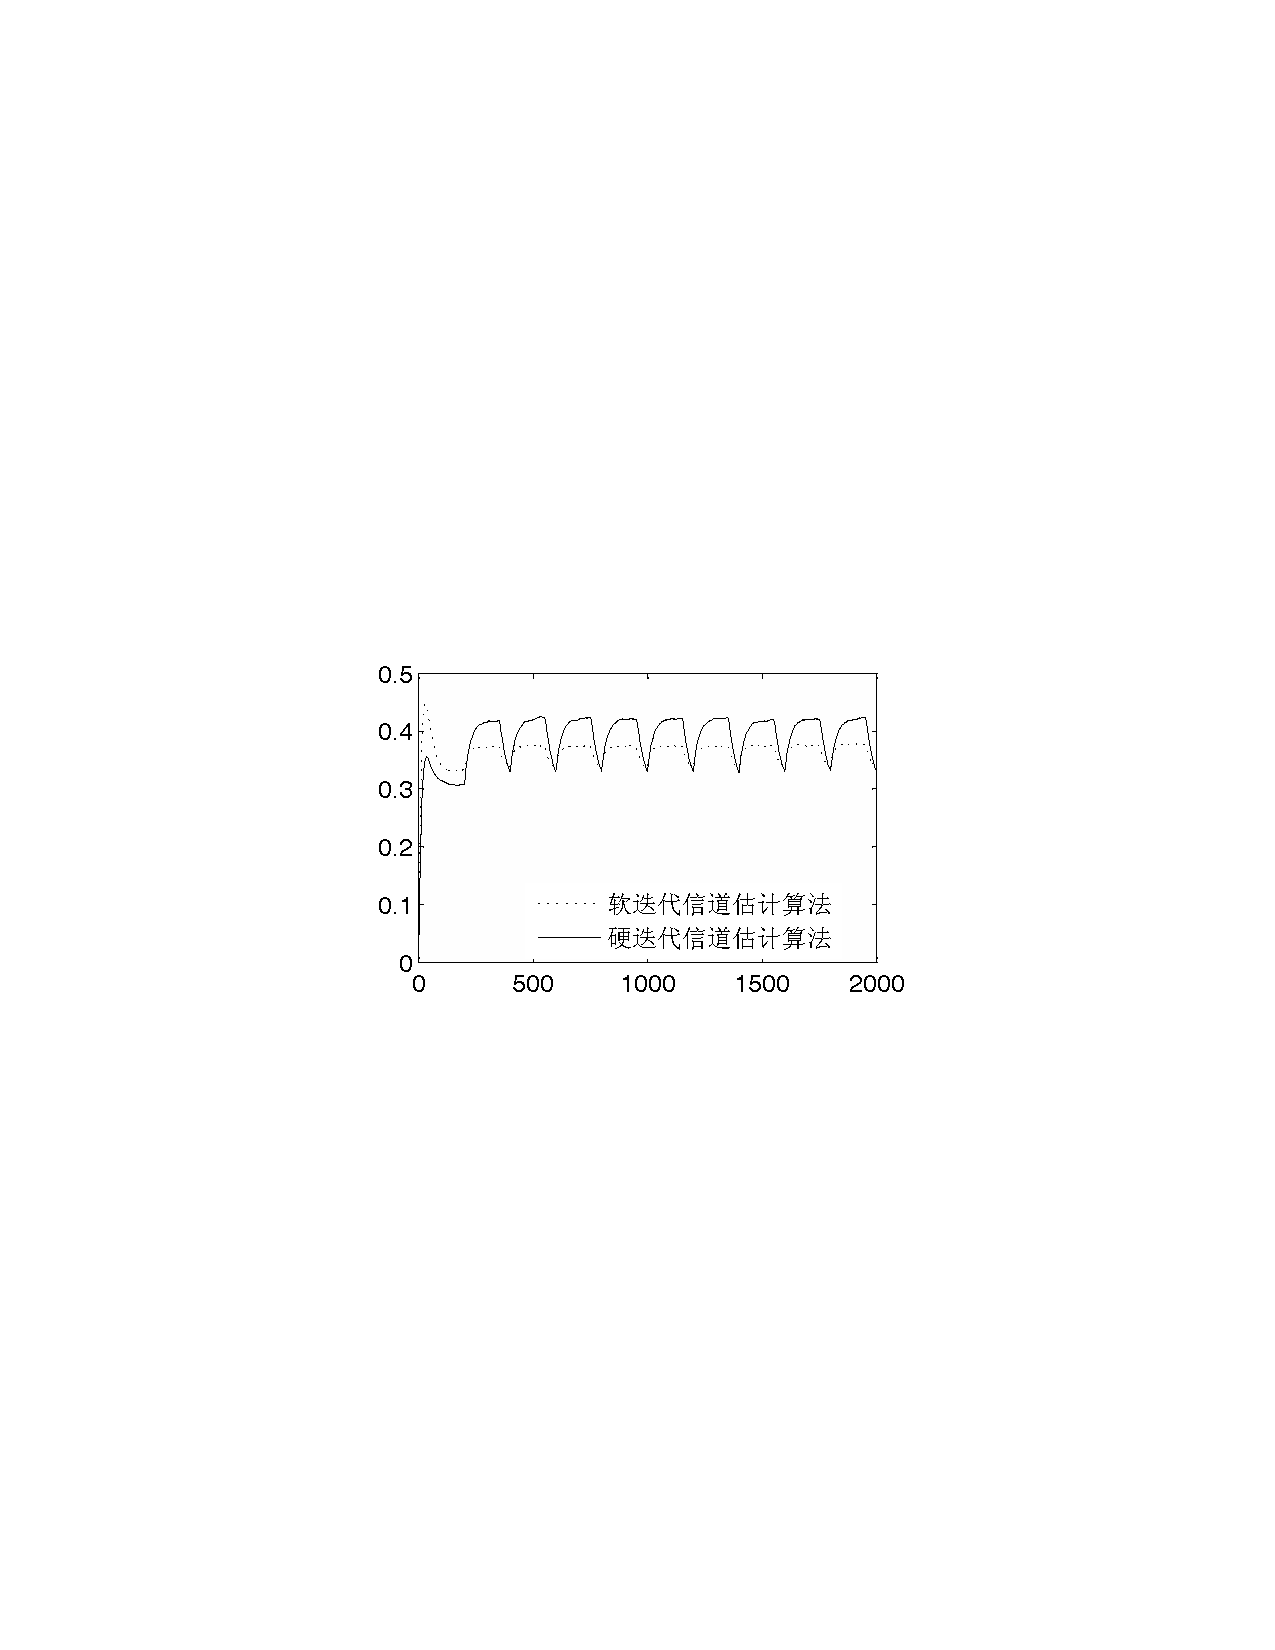
\includegraphics[width=0.5\textwidth]{images/hard_soft_3_c.pdf}
}%
    \caption{$\sigma_L=3$时硬迭代与软迭代信道估计算法比较}
    \label{fig:4.5}
\end{figure}
图\ref{fig:4.5}给出了$\sigma_L^2=3$时软迭代信道估计算法与硬迭代信道估计算法的比较。与图\ref{fig:4.4}的分析方法一样,这里也分两部分进行分析,在相位估计方面,硬迭代信道估计算法的相位估计值(不论是二阶锁相环的相位估计值还是总的相位估计值)与软迭代信道估计算法的相位估计值基本一致,这是因为$\sigma_L=3$时,外部软信息已经非常可靠,因此硬判决的符号基本与期望符号一致。而在信道方差方面,软迭代信道估计算法的方差依然小于硬迭代信道估计算法的方差,只是随着$\sigma_L$的增大,它们之间的差距越来越小。
\subsection{有无相位估计器的信道估计算法比较}
在无线电通信中,信道估计算法相比于本文基于的时变横向滤波和相位旋转信道模型没有对信道相位的变化单独考虑。图\ref{fig:4.6}给出了基于这两中信道模型的信道估计算法的比较。
\begin{figure}
    \centering
    \subfigure[硬迭代信道估计算法]{
    \centering\label{fig:4.6.a}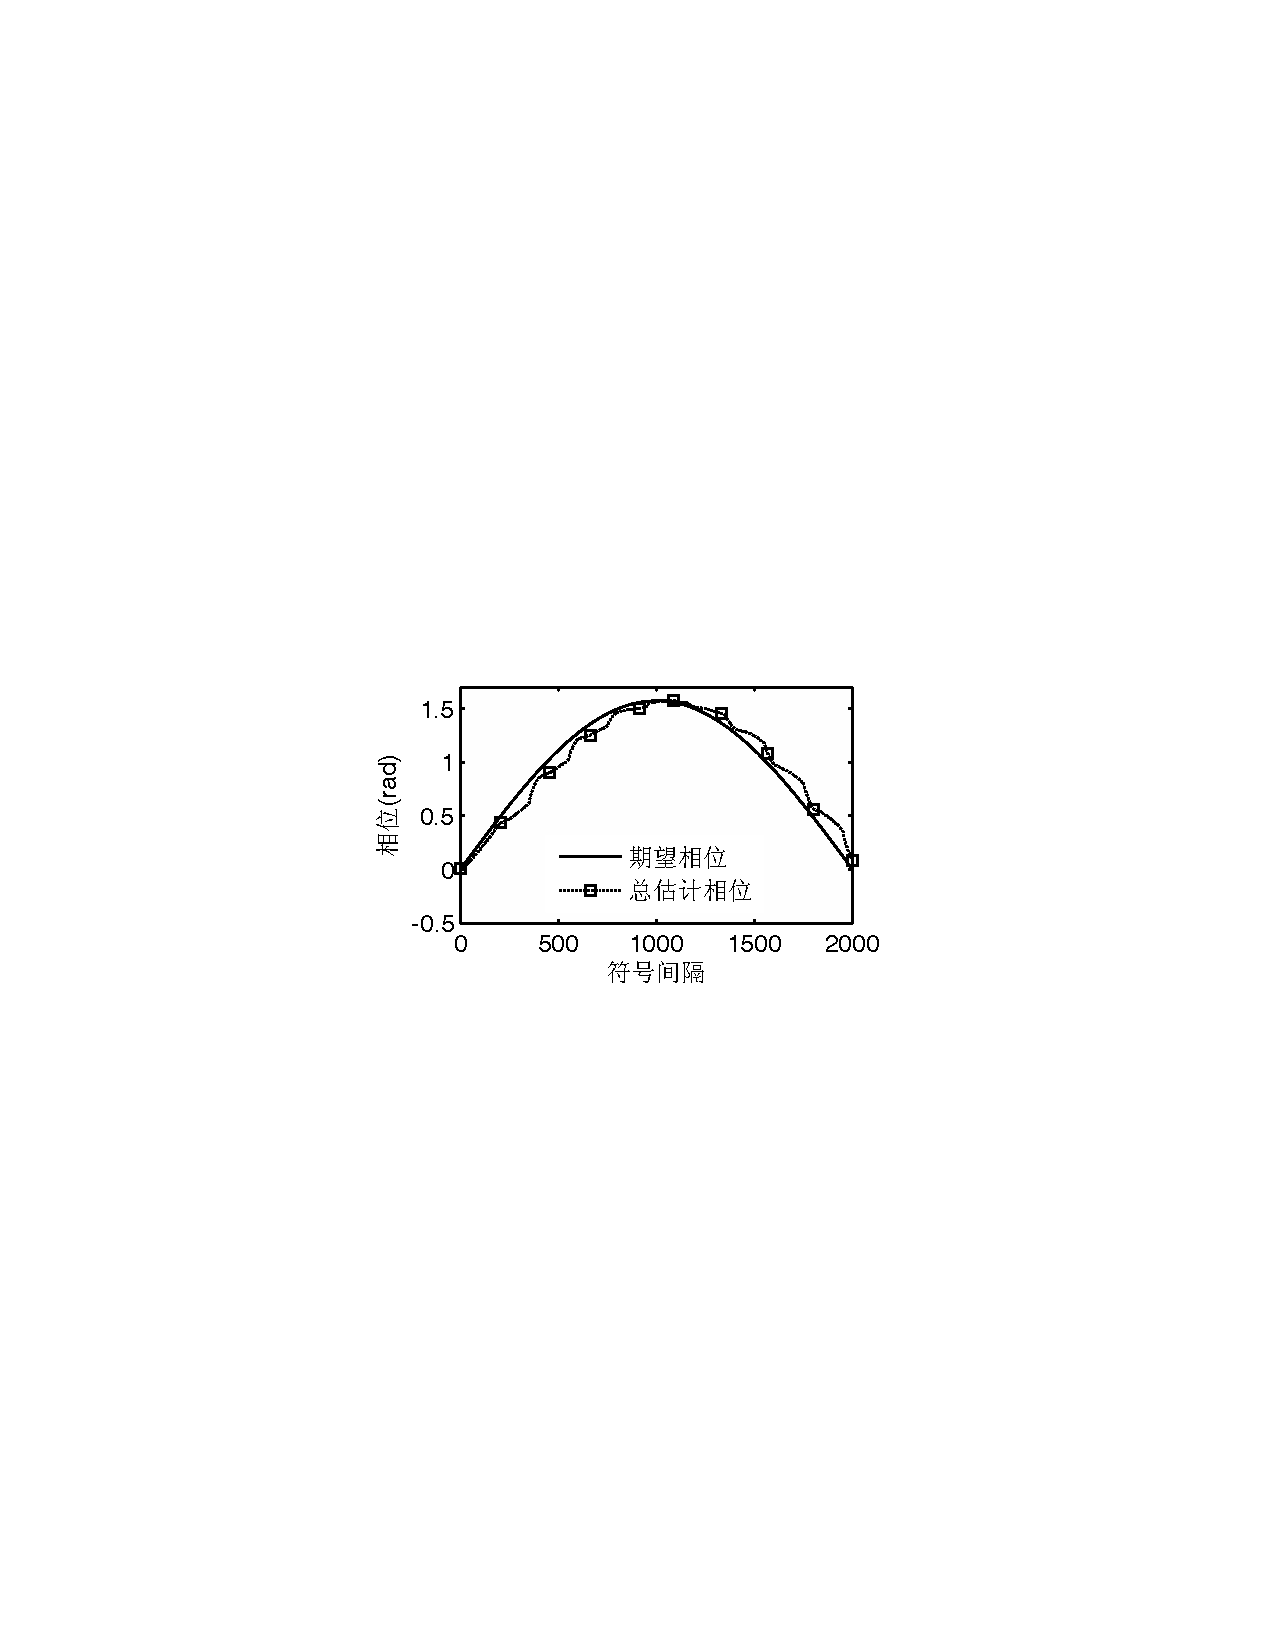
\includegraphics[width=0.45\textwidth]{images/no_phase_1_new_a.pdf}
}
    \subfigure[软迭代信道估计算法]{
    \label{fig:4.6.b}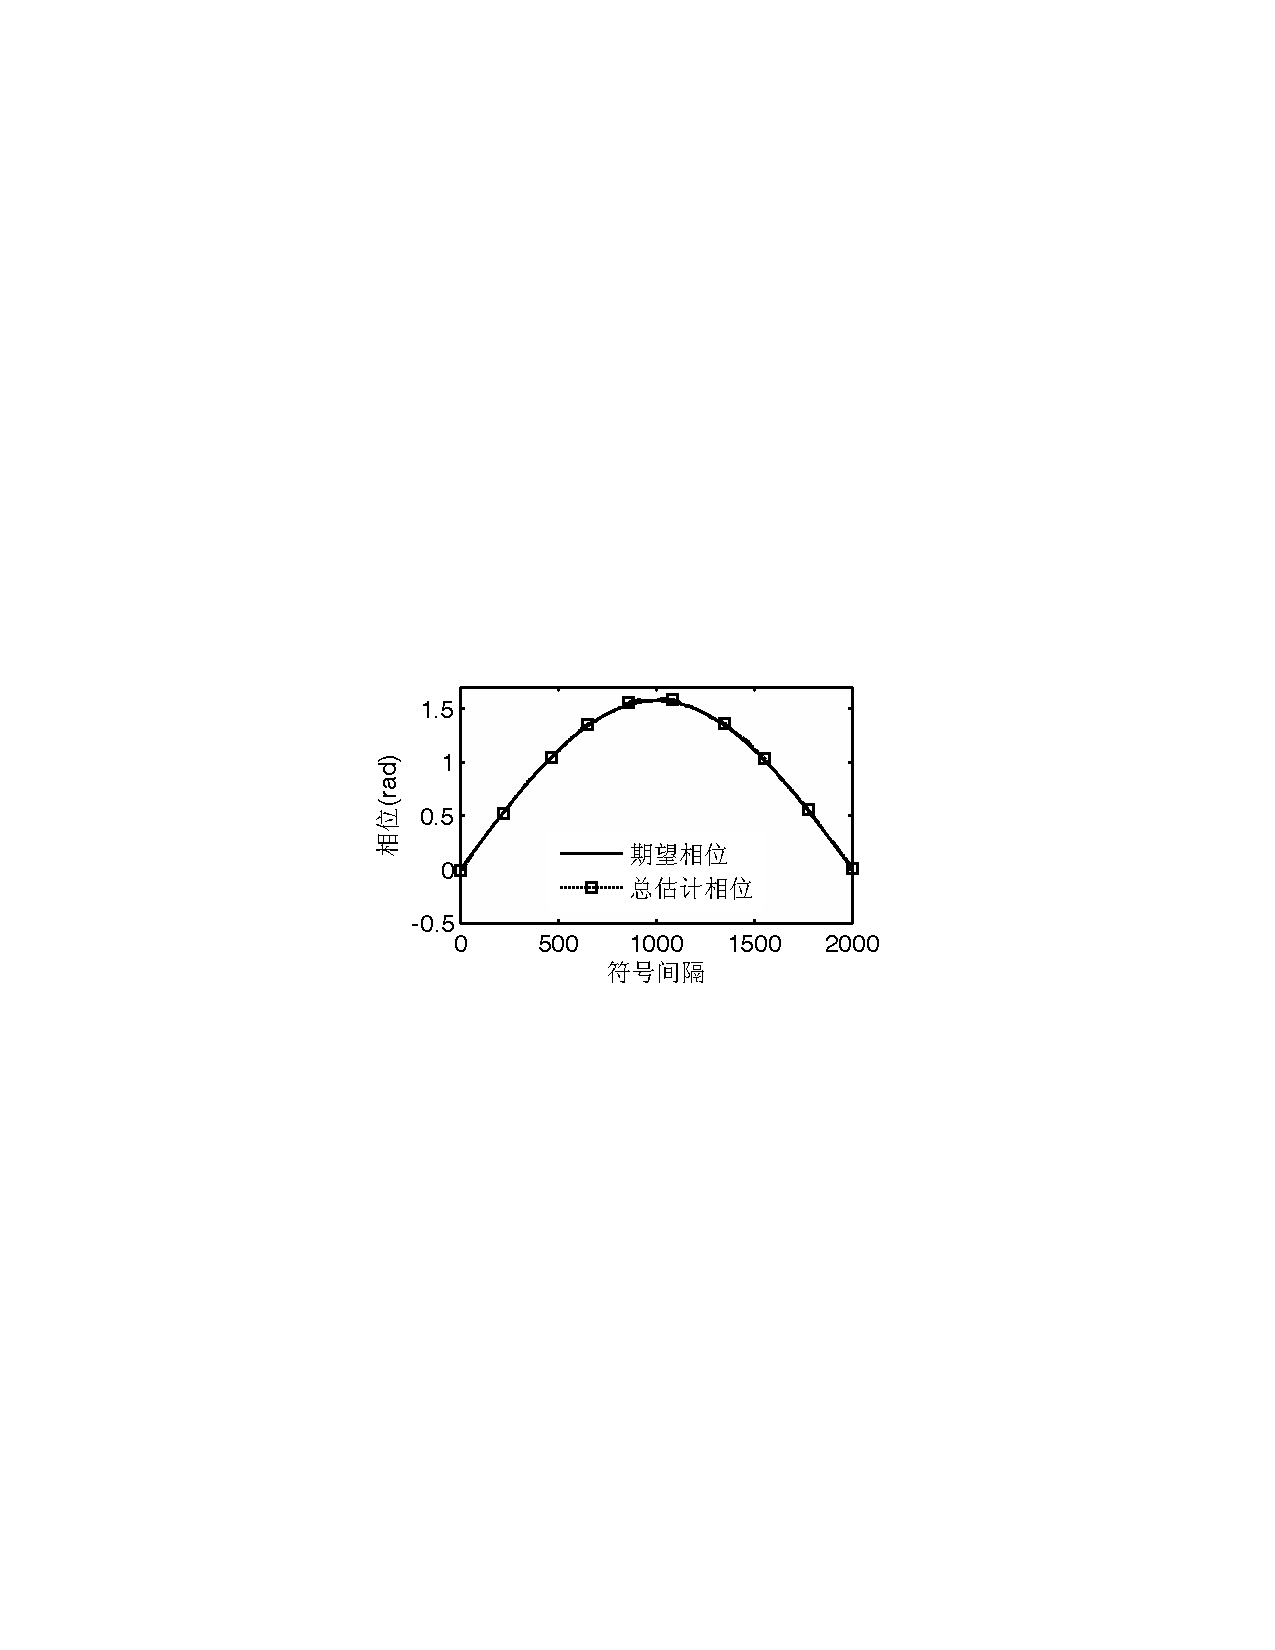
\includegraphics[width=0.45\textwidth]{images/no_phase_1_new_b.pdf}
}\\
    \subfigure[信道方差估计]{
    \label{fig:4.6.c}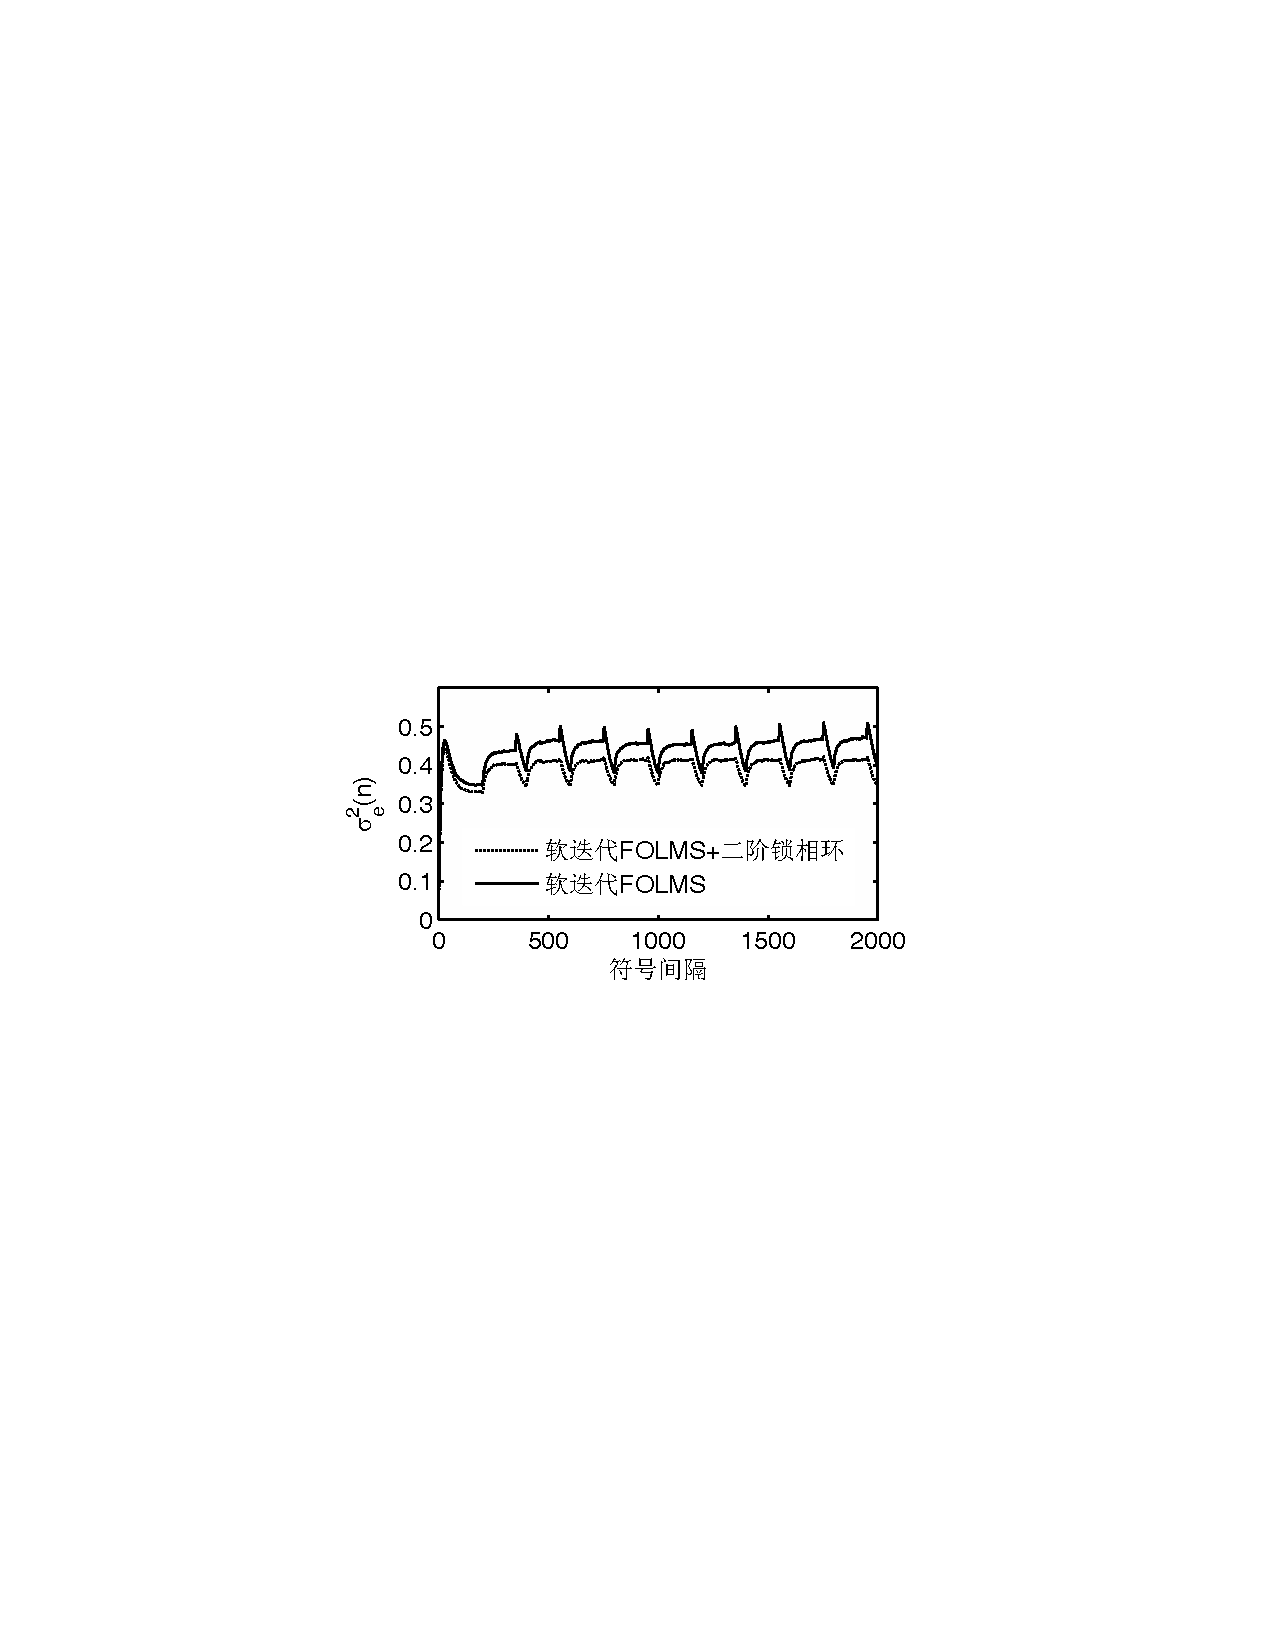
\includegraphics[width=0.5\textwidth]{images/no_phase_1_new_c.pdf}
}%
    \caption{$\sigma_L=1$时有无相位估计器的信道估计算法比较}
    \label{fig:4.6}
\end{figure}
比较图\ref{fig:4.6}(a)和图\ref{fig:4.6}(b),带相位估计器的软迭代信道估计算法的相位跟踪与估计能力要明显好于不带相位估计器的软迭代信道估计算法。而图\ref{fig:4.6}(c)从估计信道方差估计的角度可以看出,带相位估计器的软迭代信道估计算法比不带相位估计器的软迭代信道估计算法的方差小。

\begin{figure}
    \centering
    \subfigure[硬迭代信道估计算法]{
    \centering\label{fig:4.7.a}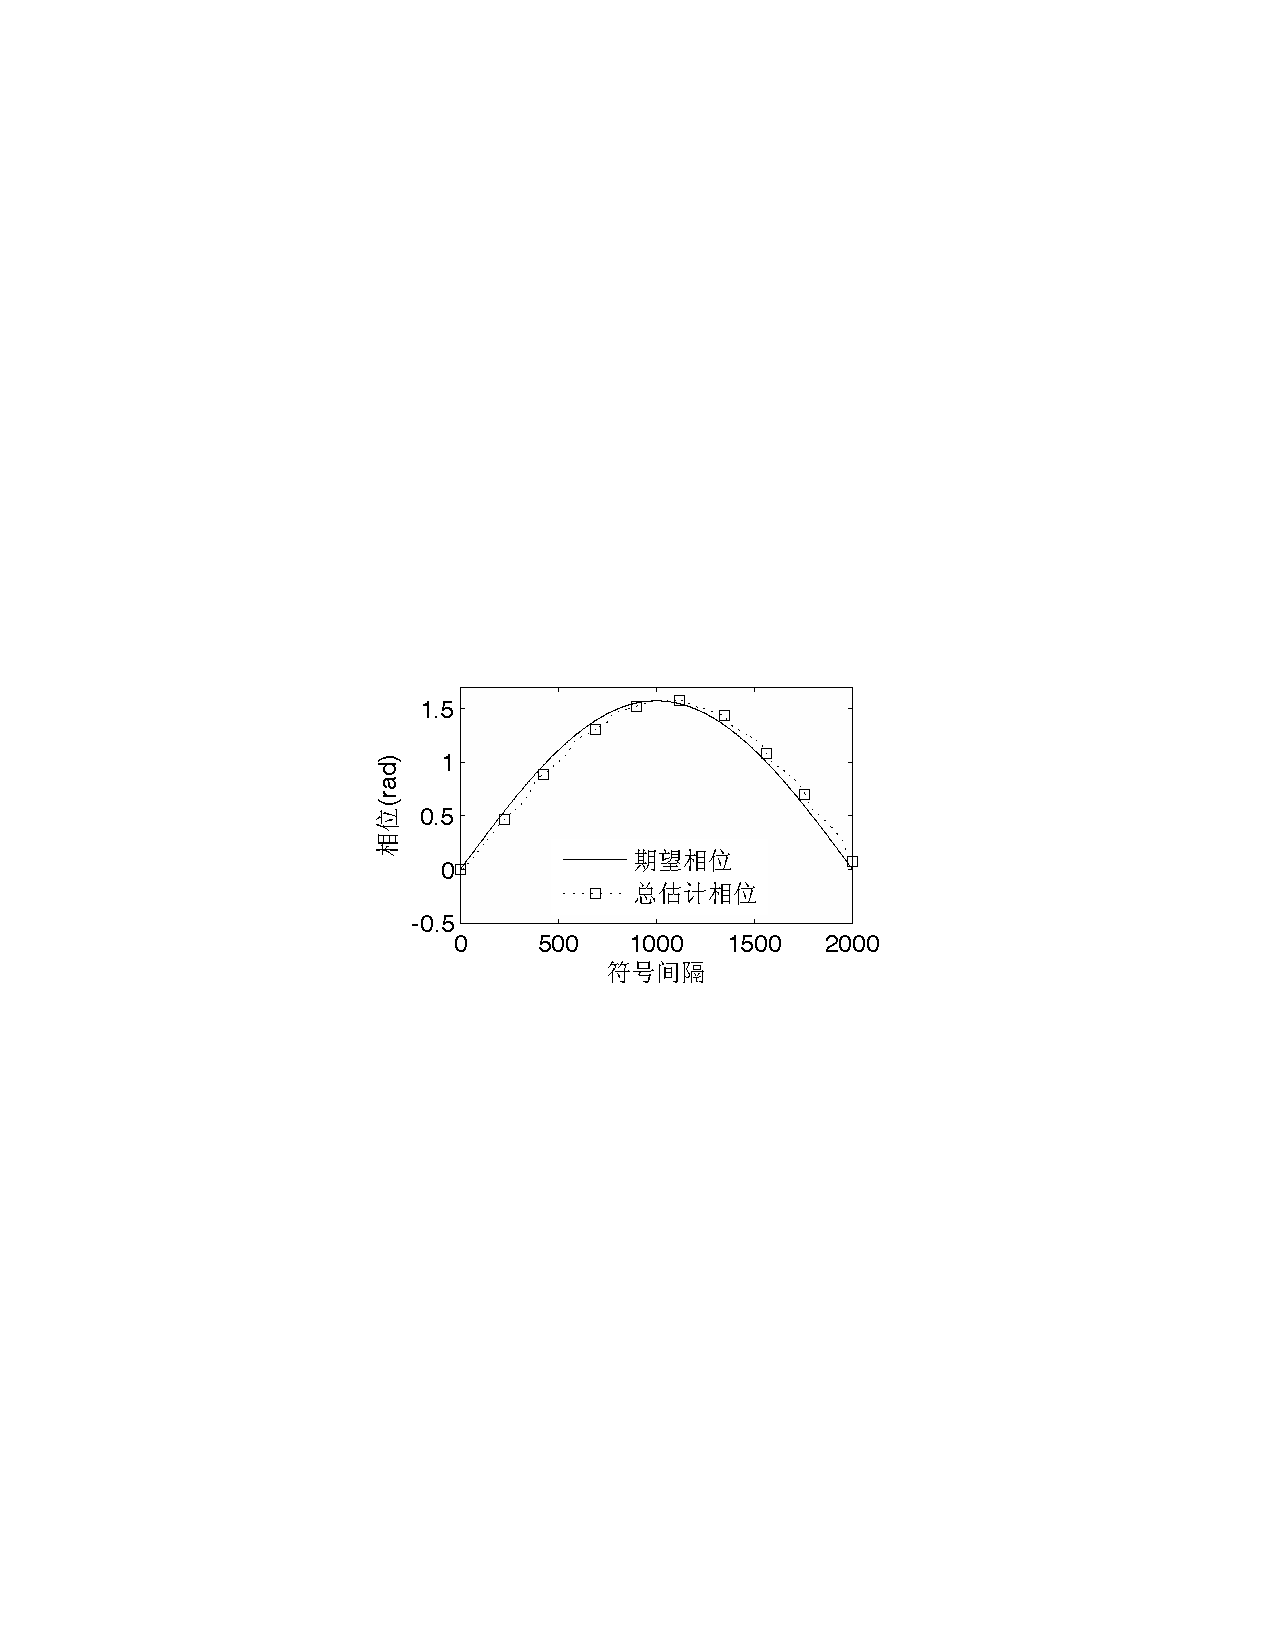
\includegraphics[width=0.45\textwidth]{images/no_phase_3_new_a.pdf}
}
    \subfigure[软迭代信道估计算法]{
    \label{fig:4.7.b}\includegraphics[width=0.45\textwidth]{images/no_phase_3_new_b.pdf}
}\\
    \subfigure[信道方差估计]{
    \label{fig:4.7.c}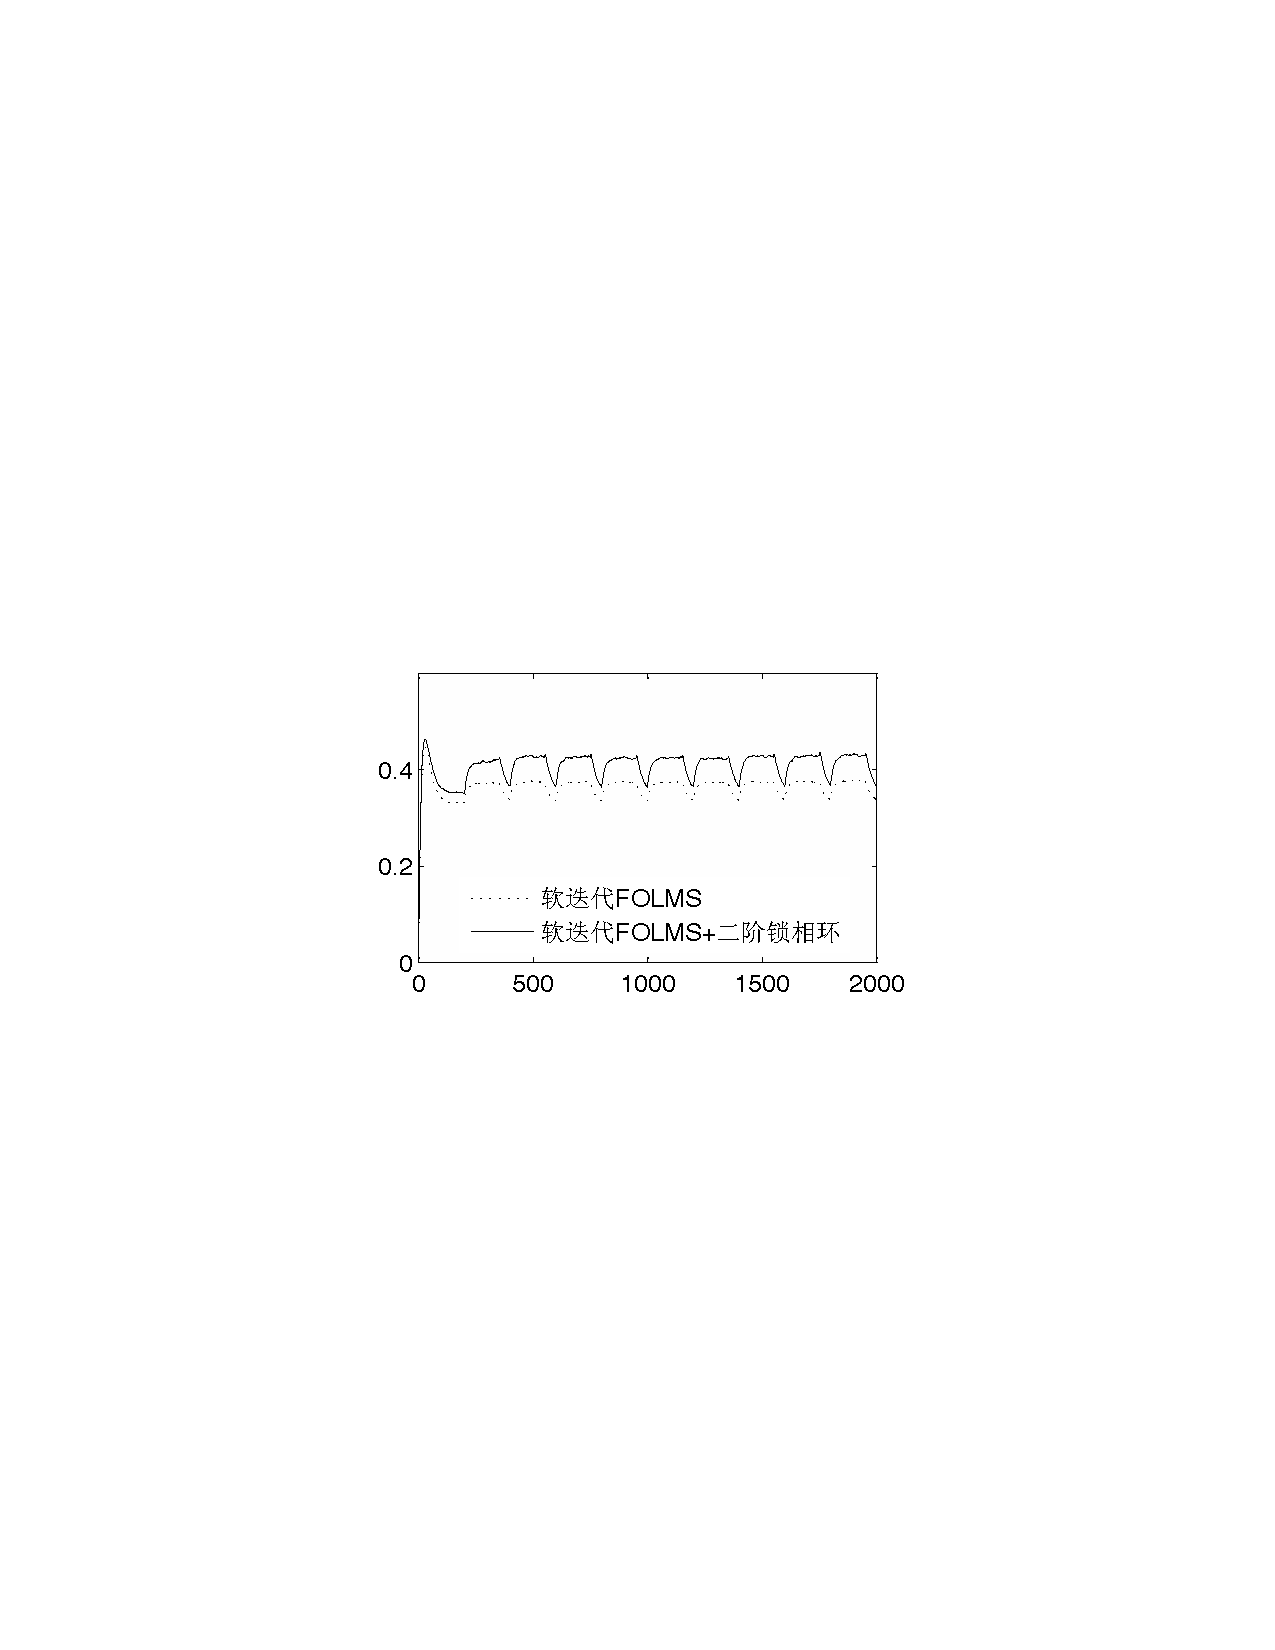
\includegraphics[width=0.5\textwidth]{images/no_phase_3_new_c.pdf}
}%
    \caption{$\sigma_L=3$时有无相位估计器的信道估计算法比较}
    \label{fig:4.7}
\end{figure}
图\ref{fig:4.7}给出了$\sigma_L=3$时有无相位估计器的信道估计算法比较。从图中可以看出,虽然$\sigma_L$增加了,外部信息变得更可靠了,但是没有相位估计器的信道估计算法的相位估计的能力依然差于带有相位估计器的信道估计算法。单从这一点出发,就应该选择带有相位估计器的信道估计算法作为水声通信系统中信道估计算法,而信道方差的估计性能更坚定了这一选择。
\section{海试数据处理}
为了验证本章提出的软迭代信道估计与相位估计联合算法对水声信道的估计性能,本文对7000m载人潜水器20110730002719海试数据进行处理并分析。此数据的产生条件为:通信距离为5570m,潜水器在海底附近,潜水器深度为5180m,声呐阵入水深度为150m,潜器与声呐的水平距离为2393m,垂直距离为5030m,对数据处理时,均衡以及信道估计算法参数设定如表\ref{tab:4.2}
\begin{table}[hbt]
  \centering
  \caption{参数设定}
  \label{tab:4.2}
  \begin{threeparttable}
  \begin{tabular}{cccc}
    \hline
    编码方式&调制方式&均衡算法&信道估计与相位估计算法\\
    \hline
    Turbo&QPSK&\tabincell{c}{基于先验信息MMSE的线性均衡\\(N=20)}&\tabincell{c}{软迭代FOLMS+二阶锁相环\\(M=20)}\\
    \hline
  \end{tabular}
\end{threeparttable}
\end{table}

7000m载人潜水器传输一幅图像需要多帧数据,每一帧数据中包含200个训练符号以及1936个数据符号。本文采用对每一帧单独处理方式。图\ref{fig:4.8}(a)和图\ref{fig:4.8}(c)为每一帧数据的估计信道方差以及估计相位。从图\ref{fig:4.8}(a)中可以看出,在迭代一次的情况下,$\sigma_e^2$处于0.1附近,并且很稳定,之所以$\sigma_e^2$没有趋于零,是因为$\sigma_e^2$还包含传输信道本身噪声的方差。

图\ref{fig:4.8}(b)为第1-14帧数据的估计信道方差,由于每一帧都做单独处理,因此变化规律和第一帧基本一致。图\ref{fig:4.8}(d)给出了第1-14帧数据的估计相位,其变化规律与图\ref{fig:4.3}基本一致,但是有一点不同,图\ref{fig:4.8}(d)的相位最终没有回归到零,分析原因有两个:
\begin{itemize}
    \item
        在对水声信道进行估计时,本文基于时变横向滤波和相位旋转模型,因此,时变横向滤波器的抽头系数也带有一定的相位信息。
    \item
        图\ref{fig:4.3}的模型假定的是帧与帧之间是没有空隙的,但是在7000m载人潜水器通信系统中,帧与帧之间是有固定的时间空隙。这也一定程度上导致了图\ref{fig:4.8}(d)中相位最终没有回归到零。
\end{itemize}
\begin{figure}
    \centering
    \subfigure[第1帧数据的估计信道方差]{
    \label{fig:4.8.a}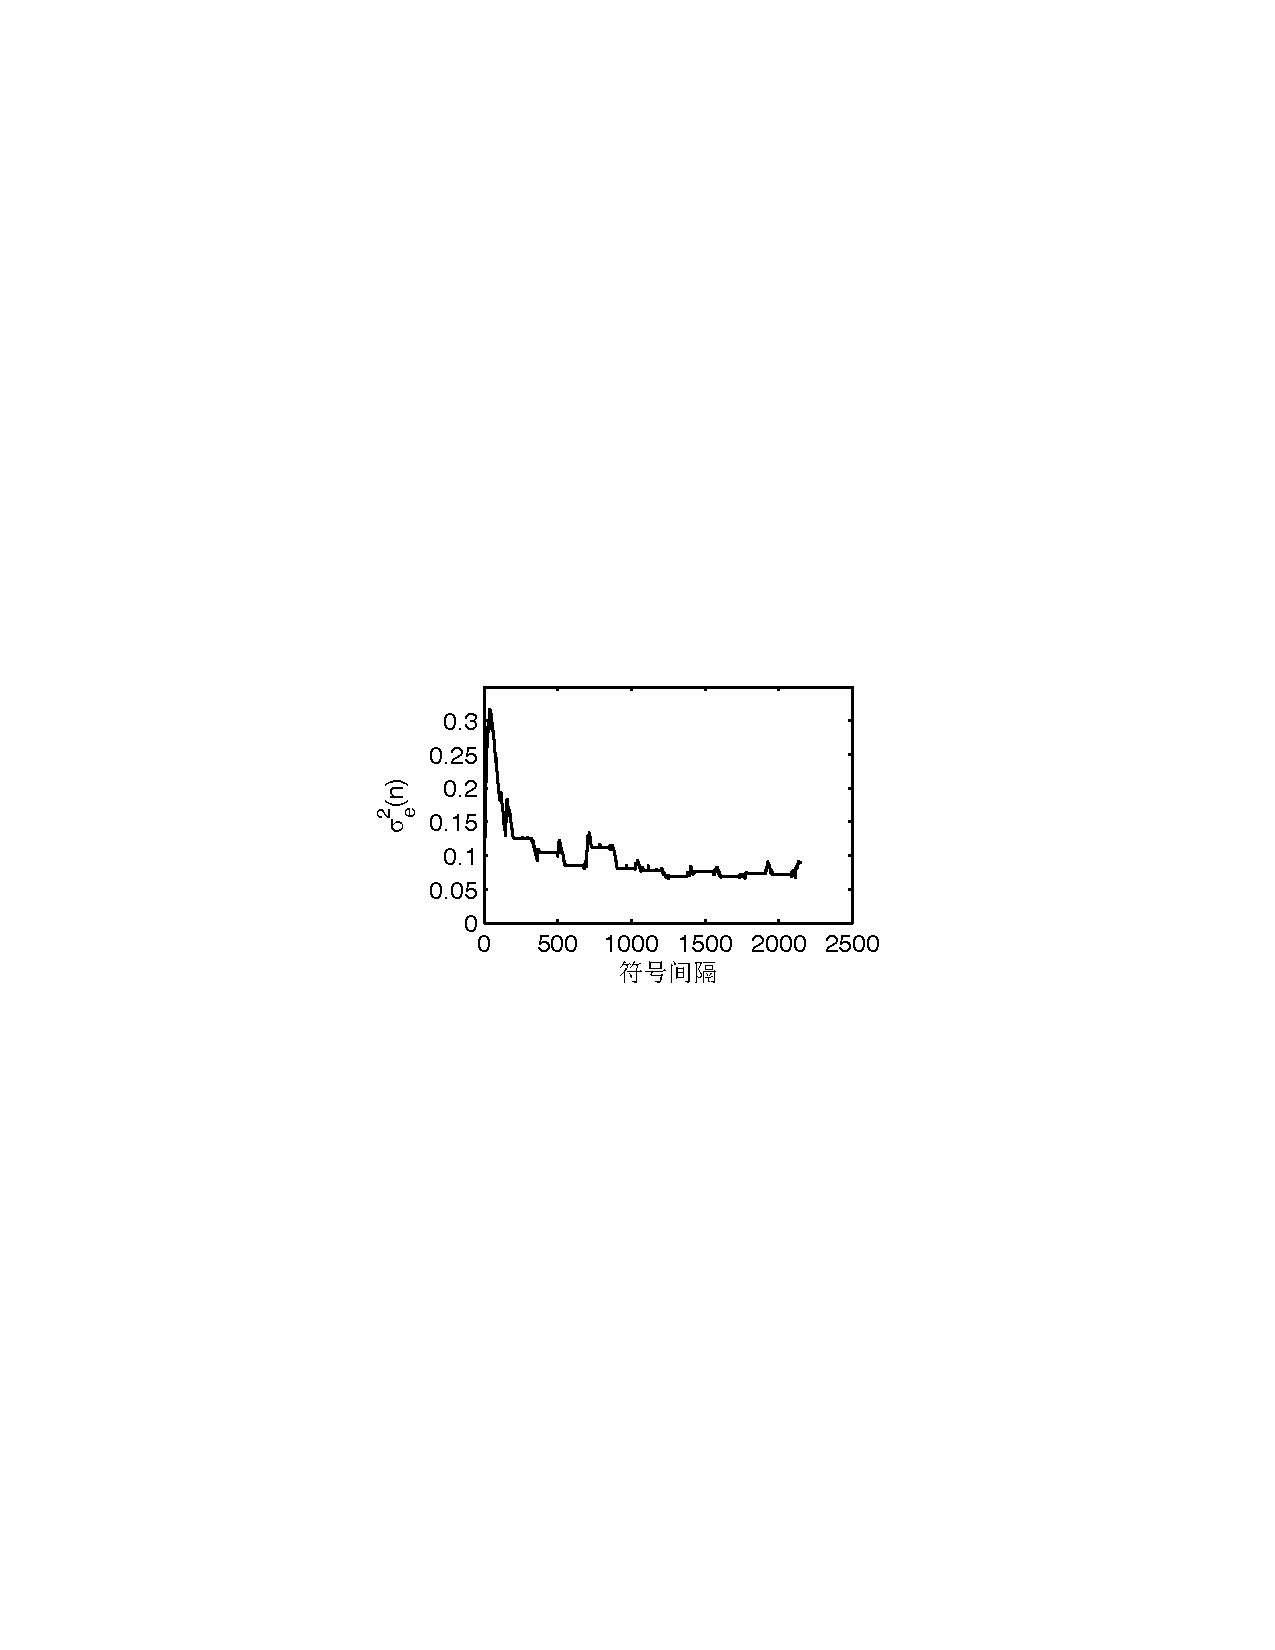
\includegraphics[width=0.45\textwidth]{images/new_paper_a.pdf}
    }\;
    \subfigure[第1-14帧数据的估计信道方差]{
    \label{fig:4.8.b}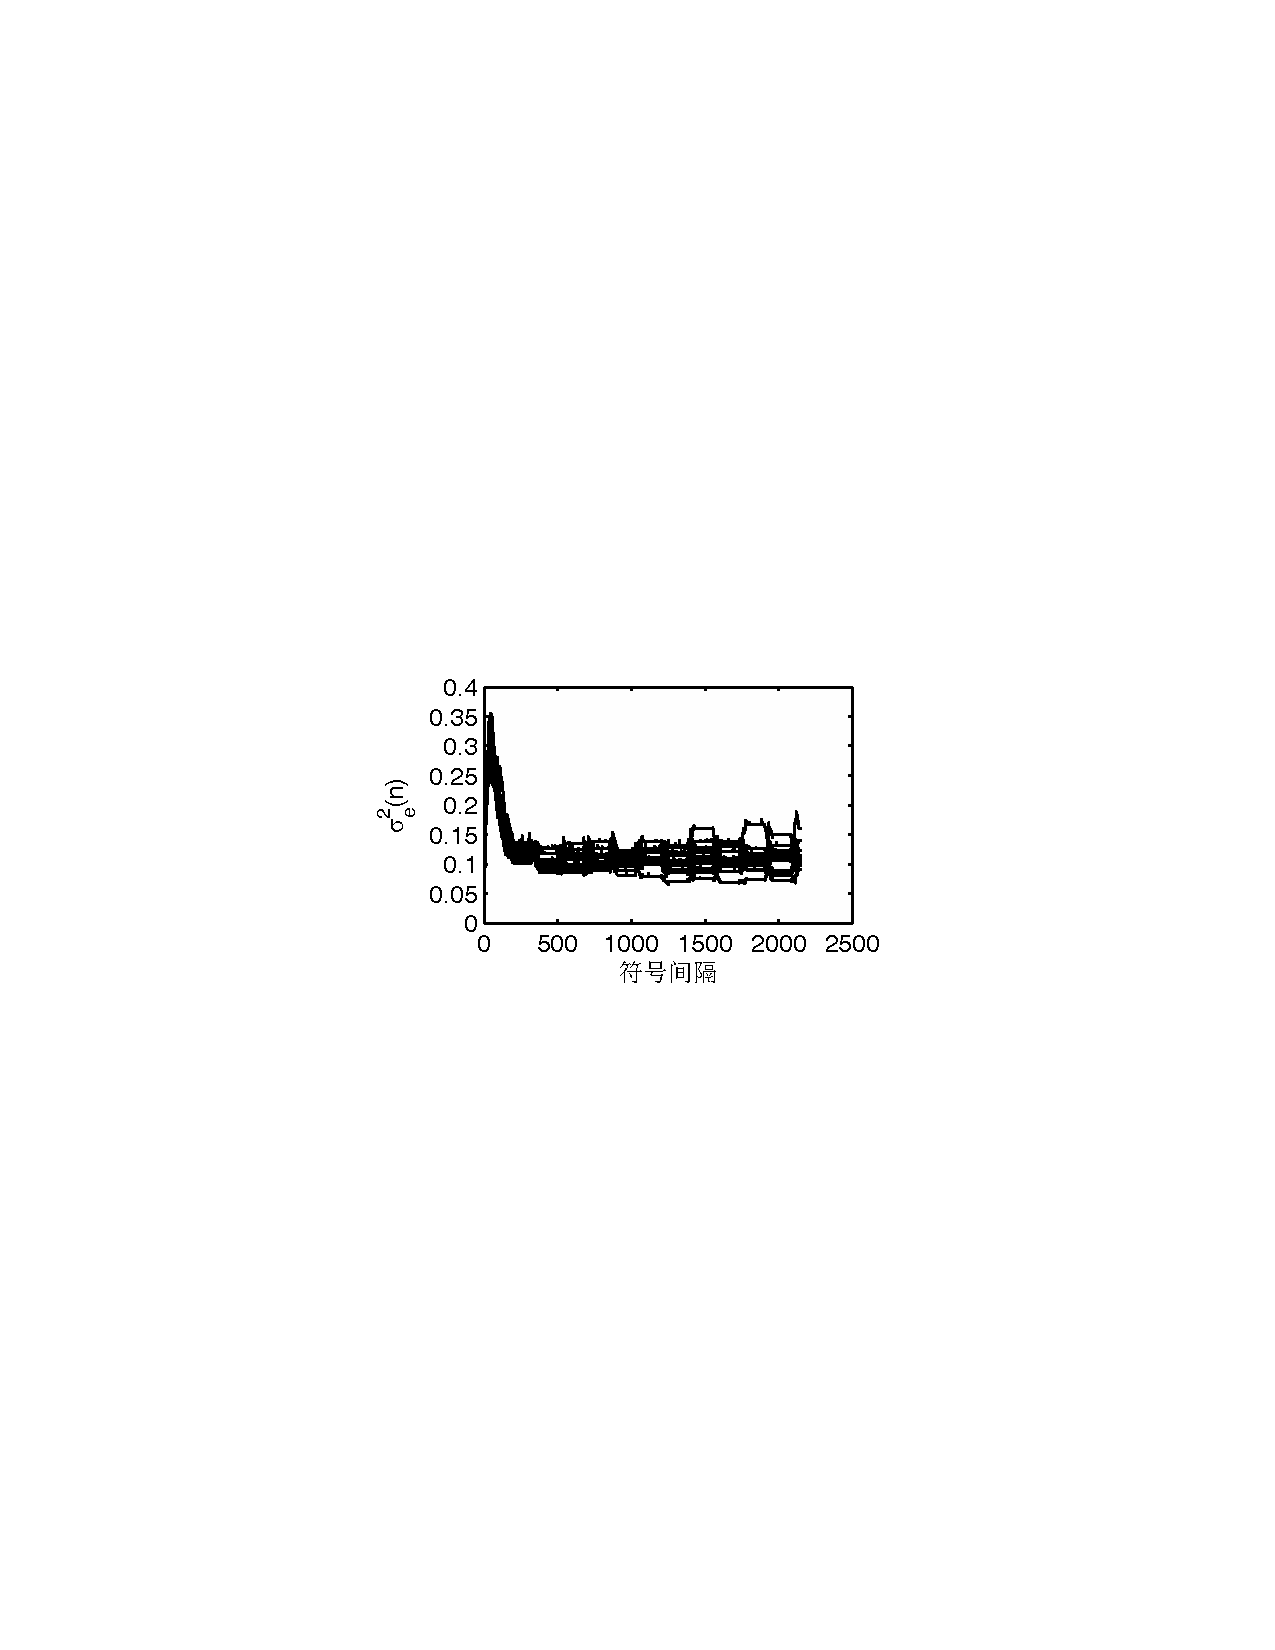
\includegraphics[width=0.45\textwidth]{images/new_paper_b.pdf}
    }\\
    \subfigure[第1帧数据的估计相位]{
    \label{fig:4.8.c}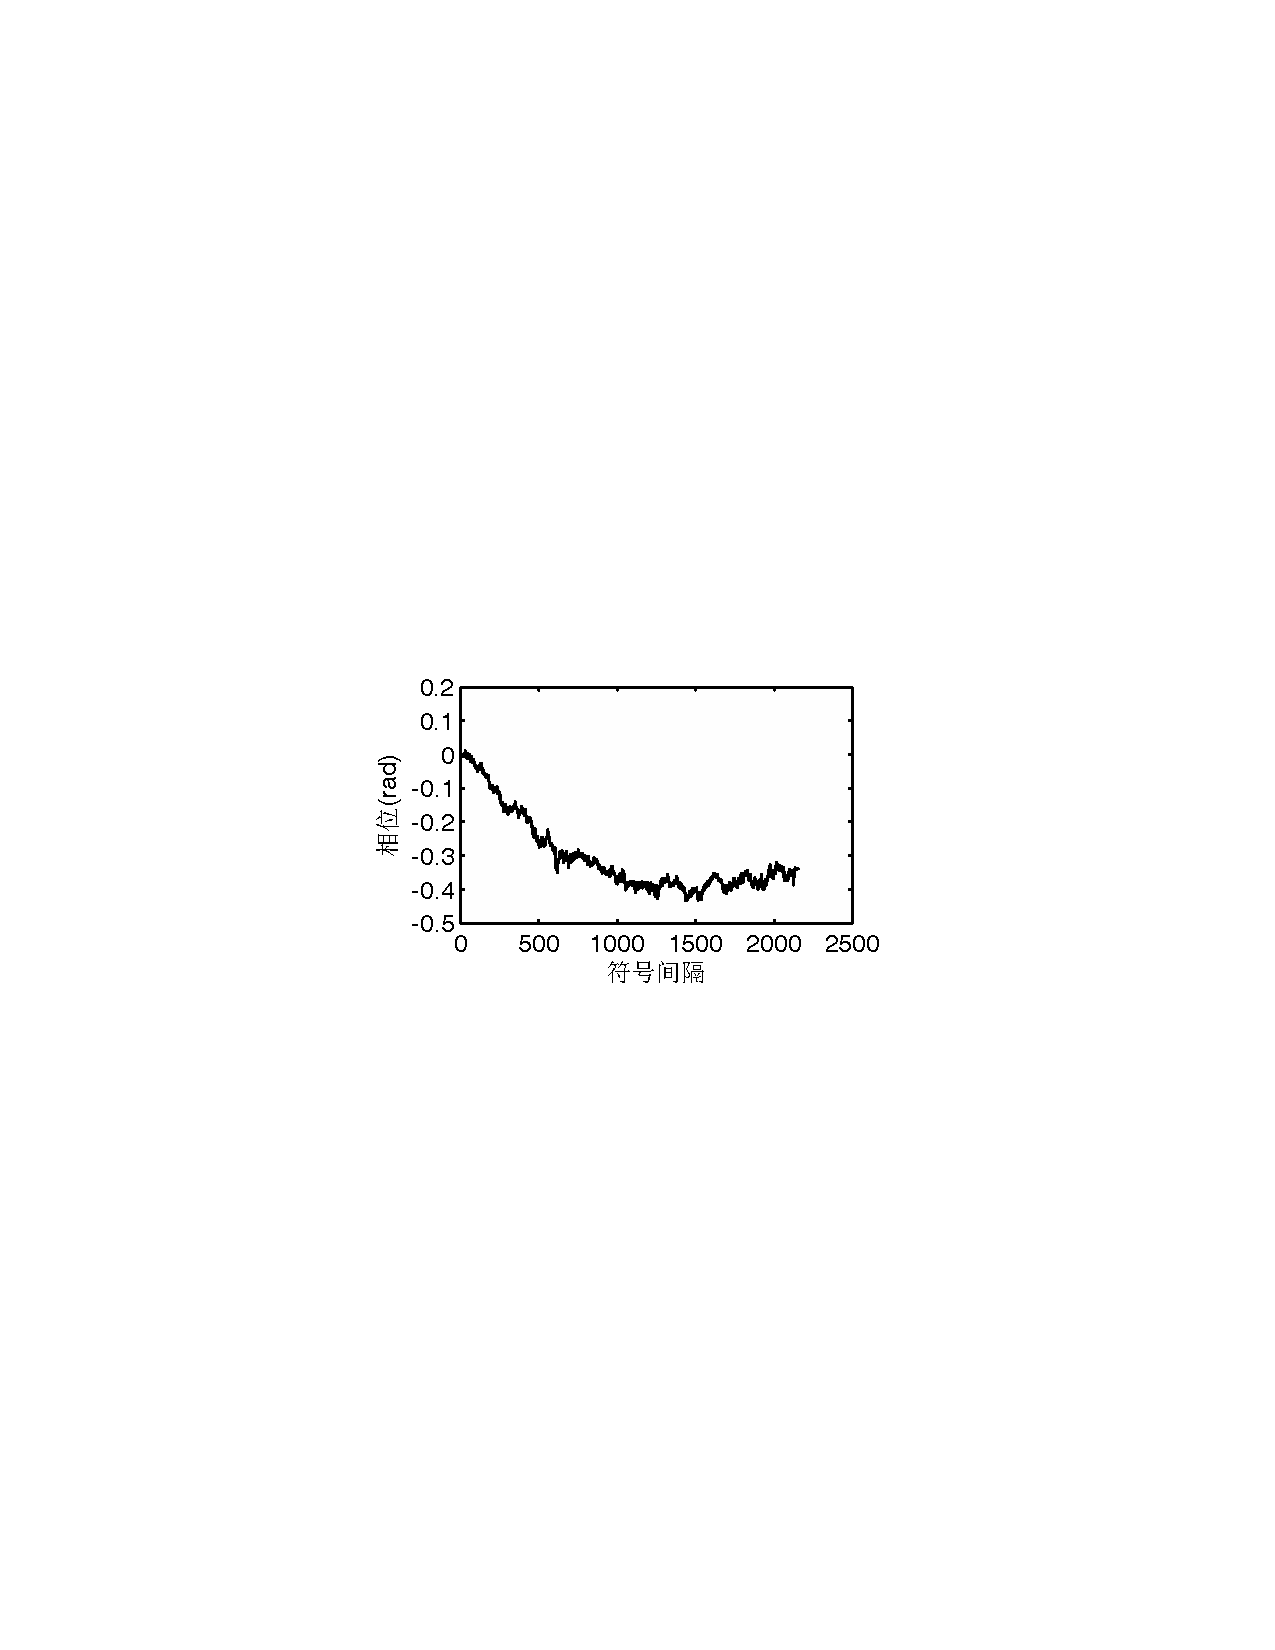
\includegraphics[width=0.45\textwidth]{images/new_paper_c.pdf}
    }\;
    \subfigure[第1-14帧数据的估计相位]{
    \label{fig:4.8.d}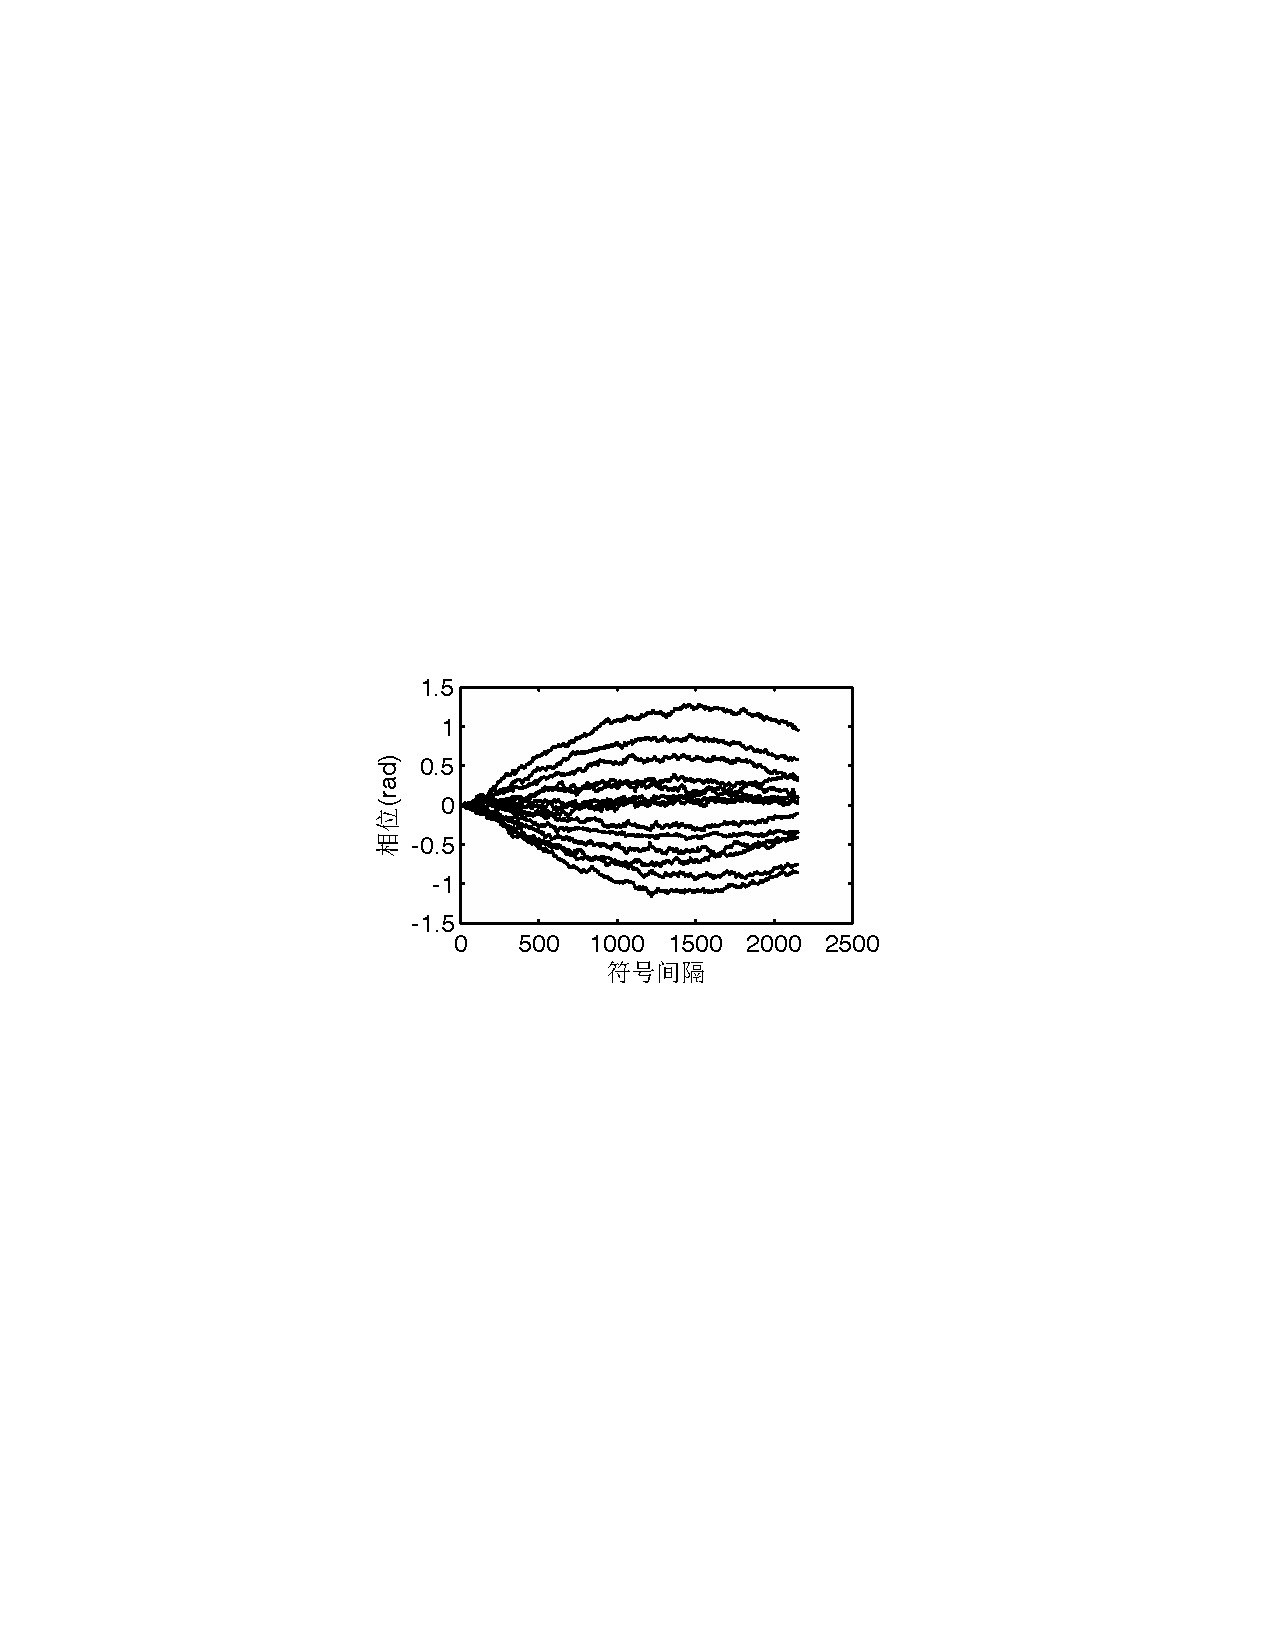
\includegraphics[width=0.45\textwidth]{images/new_paper_d.pdf}
    }
    \caption{迭代一次时信道估计误差的方差与估计相位}
    \label{fig:4.8}
\end{figure}

\begin{figure}
    \centering
    \subfigure[接收信号星座图]{
    \label{fig:4.9.a}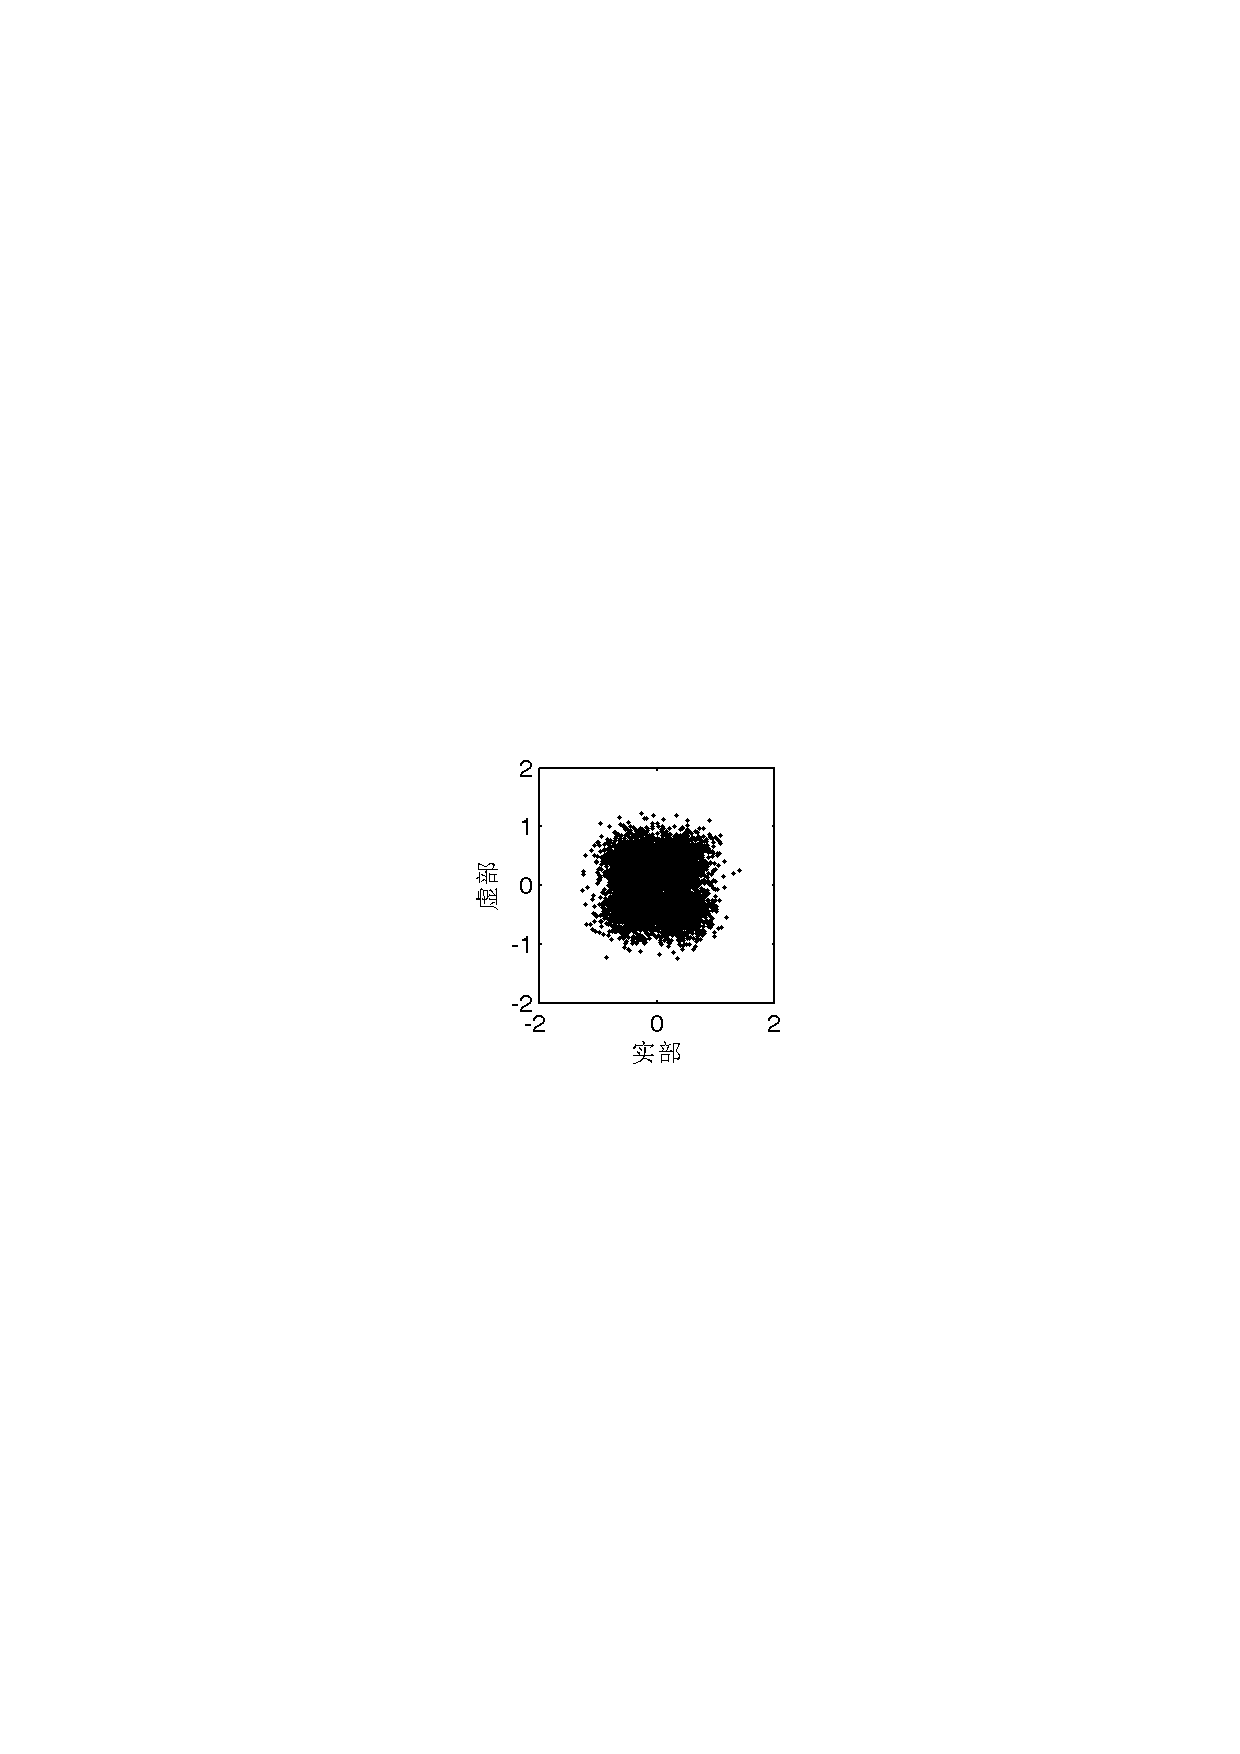
\includegraphics[width=0.45\textwidth]{images/final_1.pdf}
    }\;
    \subfigure[迭代0次均衡器输出星座图]{
    \label{fig:4.9.b}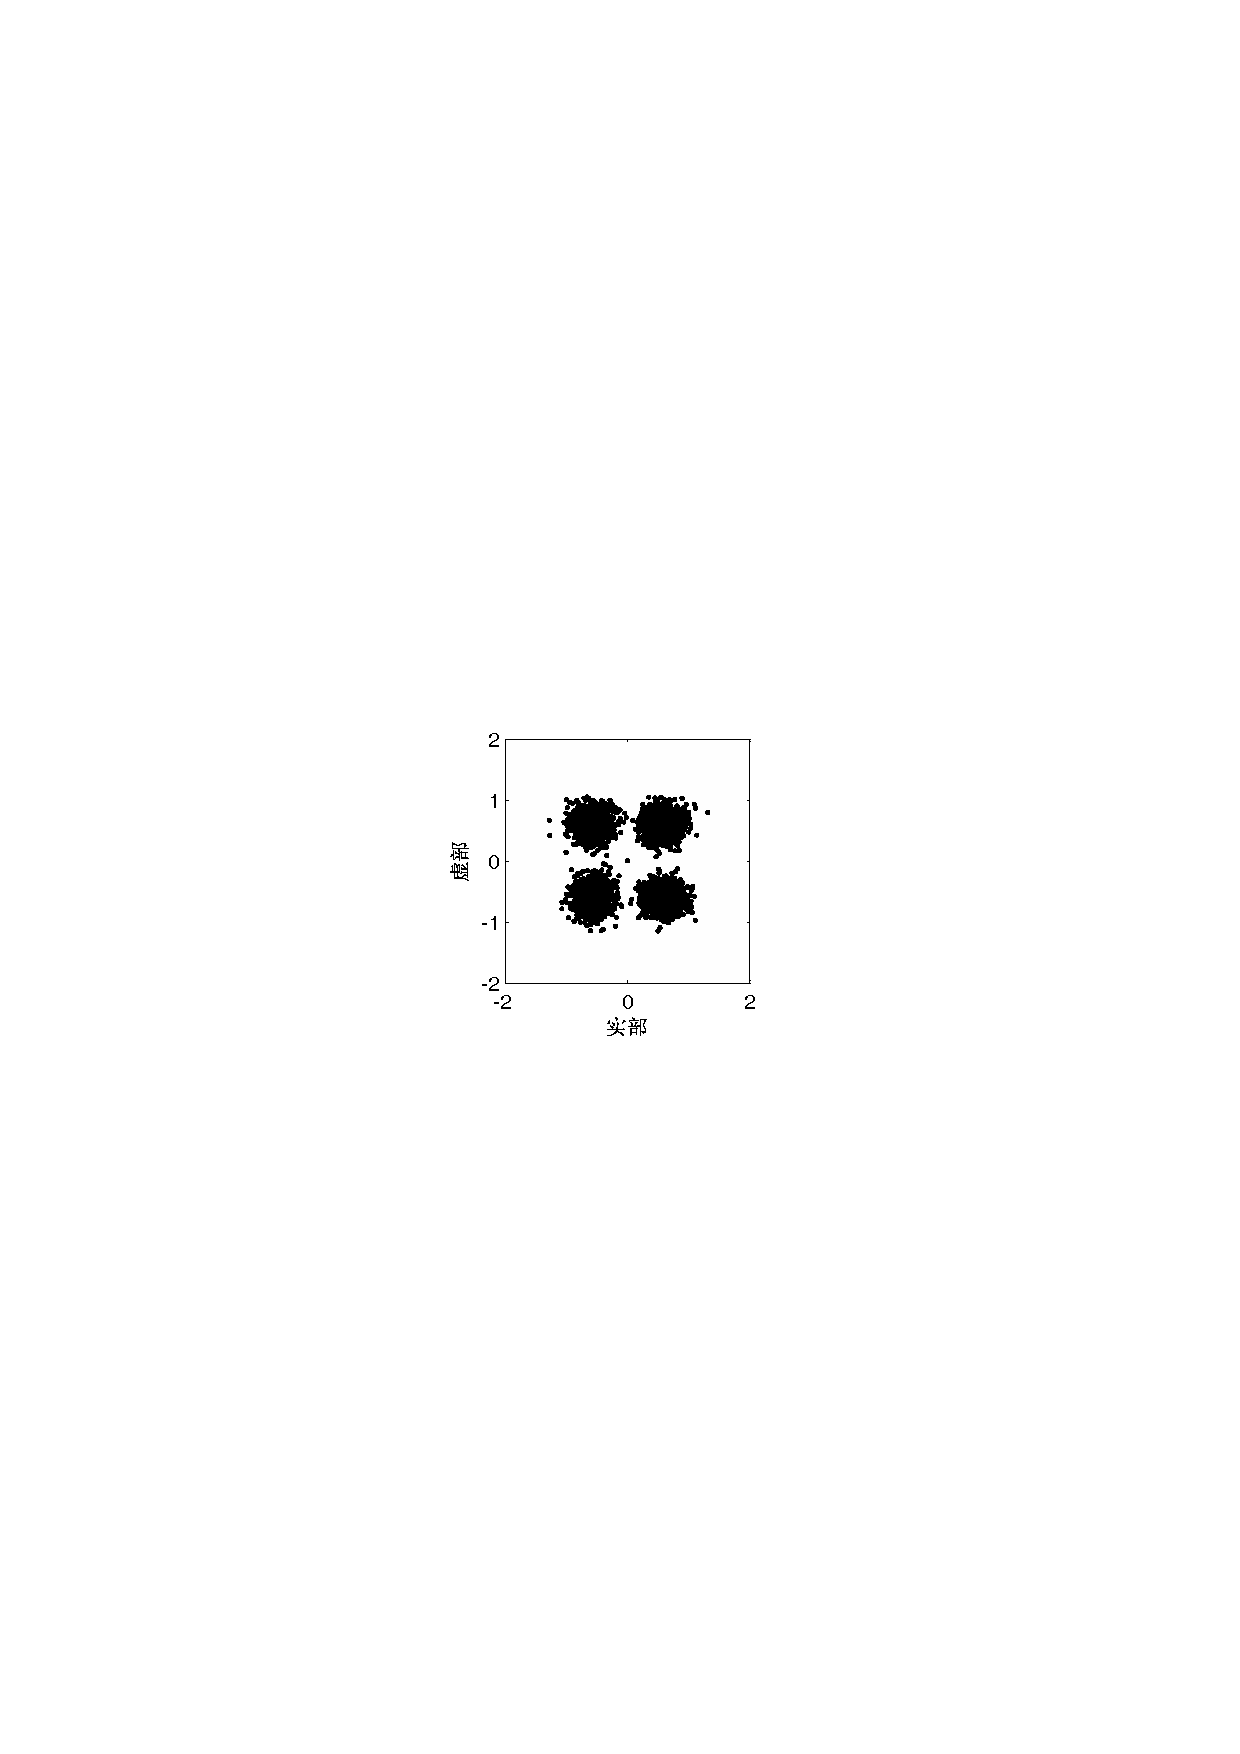
\includegraphics[width=0.45\textwidth]{images/final_2.pdf}
    }\\
    \subfigure[第1帧数据的估计相位]{
    \label{fig:4.9.c}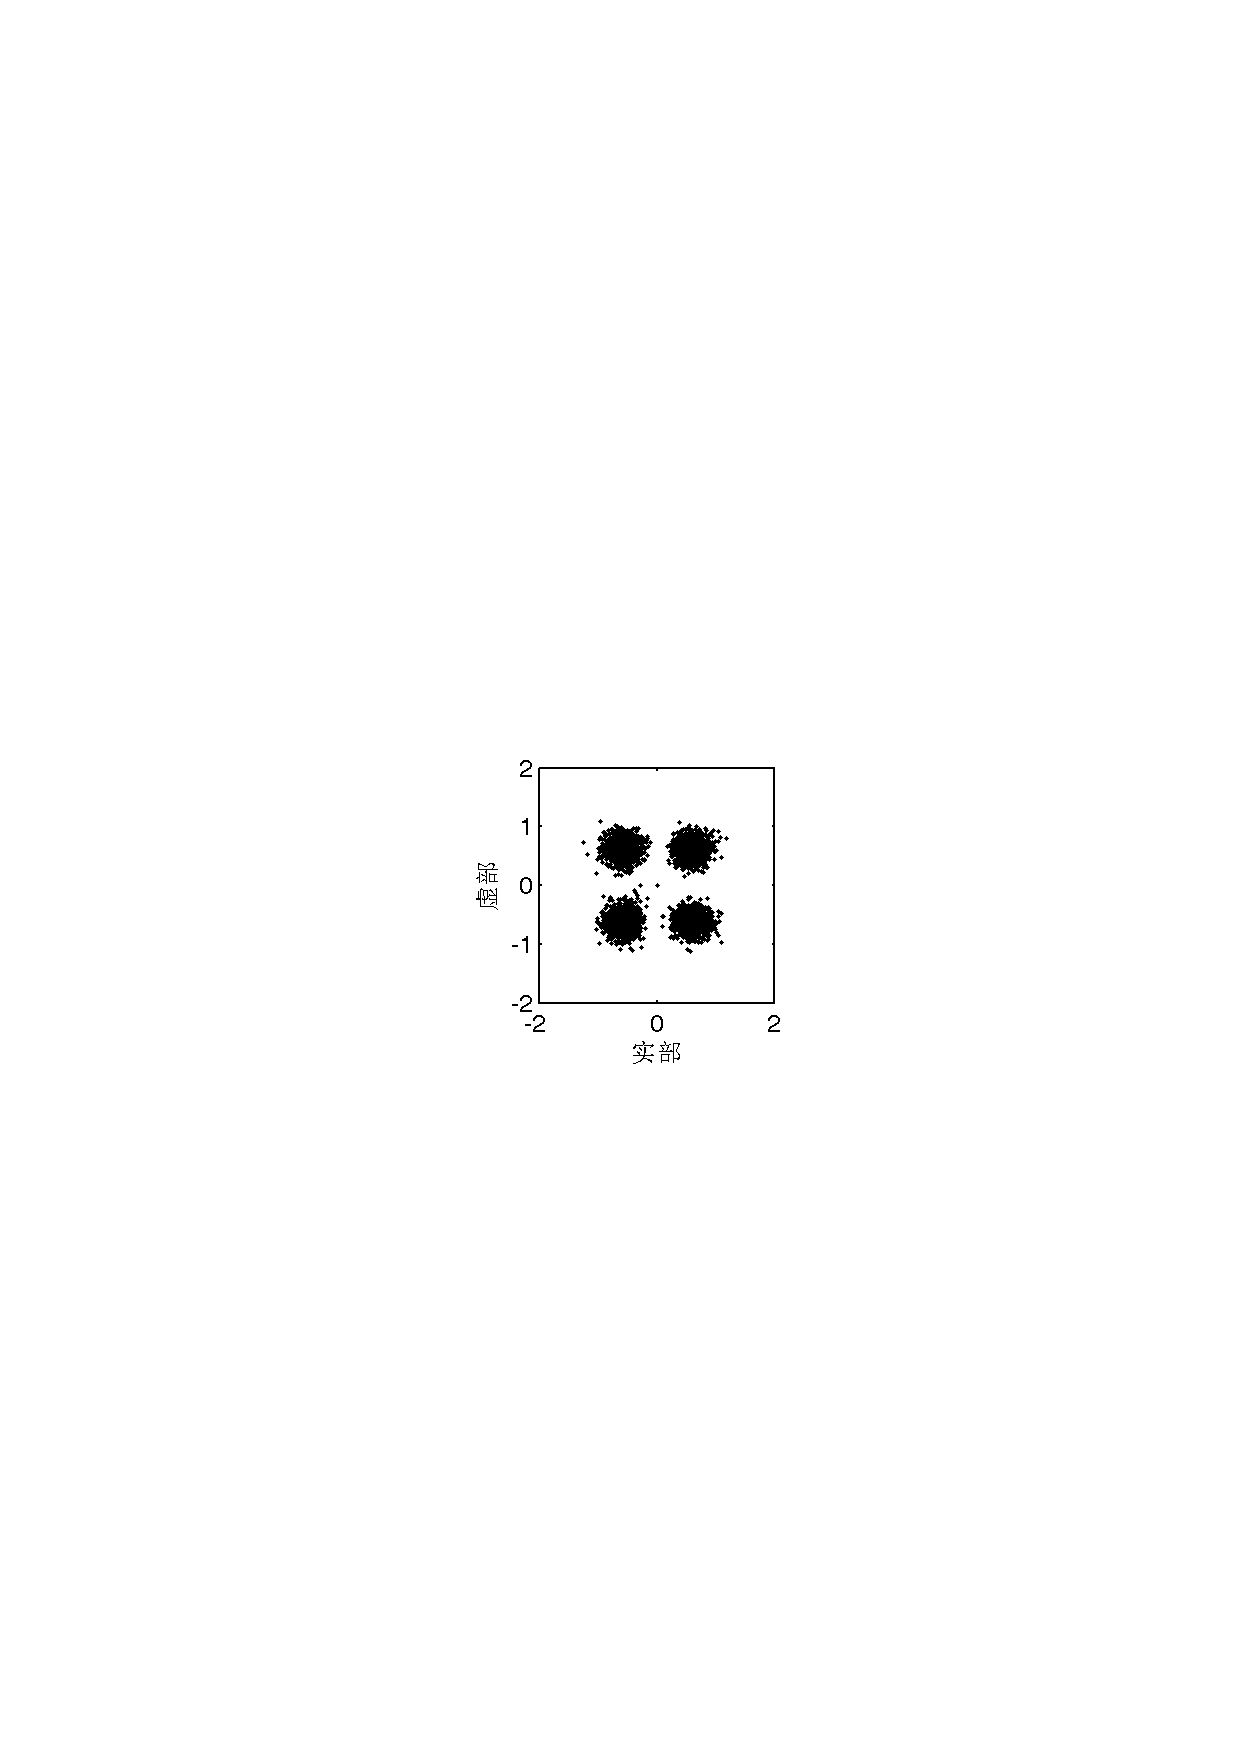
\includegraphics[width=0.5\textwidth]{images/final_3.pdf}
    }
    \caption{基于本文信道估计与相位估计算法的MMSE-TE的均衡输出星座图比较}
    \label{fig:4.9}
\end{figure}

通过图\ref{fig:4.9}(a),图\ref{fig:4.9.b}以及图\ref{fig:4.9}(c)的基于本文信道估计与相位估计算法的MMSE-TE的均衡输出星座图比较可以看出,随着迭代次数的增加,均衡器的性能越好,当迭代一次时,均衡器输出信息经过Turbo译码器可以实现无差错译码。
%==========================================================================
\section{本章小结}
针对水声通信信道相位时变的特性,本文在文献\ncite{Otnes2004}的基础上提出一种Turbo均衡中的软迭代信道估计算法。该算法采用软迭代快速自优化LMS跟踪和更新信道冲击响应,以及二阶锁相环跟踪和估计相位变化,软迭代信道估计算法相比于本文介绍的其他算法,在不增加运算量的前提下,改善了信道估计的收敛速度并提供良好的相位估计能力。由仿真结果可知,本文提出的软迭代信道估计算法的信道估计与相位估计的性能明显优于硬迭代信道估计与相位估计联合算法,在相位估计方面,本文提出的软迭代信道估计算法的性能远远优于不带相位估计器的软迭代信道估计算法。从海试数据处理中可以看出,本文提出的算法能够为Turbo均衡器提供可靠地时变横向滤波器系数矢量、各个符号处的相位以及信道方差,从而大大提高Turbo均衡器的性能。
%==========================================================================
%%========================================================================
% empty page for two-page print
\ifthenelse{\equal{\ioaside}{T}}{%
  \newpage\mbox{}%
  \thispagestyle{empty}}{}
%%========================================================================
%\end{document}
